\section{Additional Visualizations and Experiments for \methodname}

In this section, we provide visualizations and diagnostic experiments evaluating various  aspects of feature co-adaptation and the \methodname\ regularizer. We first provide more empirical evidence showing the presence of feature co-adaptation in modern deep offline RL algorithms. We will also visualize \methodname\, inspired from the implicit regularizer term in TD-learning alleviates rank collapse discussed in \citet{kumar2021implicit}. We will compare the efficacies of the explicit regularizer induced for different choices of the noise covariance matrix $M$ (Equation~\ref{eqn:regularizer}), understand the effect of dropping the stop gradient term in ou practical regularizer and finally, perform diagnostic experiments visualizing if the Q-networks learned with DR3 resemble more like neural networks trained via supervised learning, measured in terms of sensitivity and robustness to layer reinitialization~\citep{zhang2019all}.

\vspace{-0.05in}
\subsection{More Empirical Evidence of Feature Co-Adaptation}
\label{app:more_evidence_coadaptation}
In this section, we provide more empirical evidence demonstrating the existence of the feature co-adaptation issue in modern offline RL algorithms such as DQN and CQL. As shown below in Figure~\ref{fig:dot_product_increases_five_games}, while the average dataset Q-value for both CQL and DQN exhibit a flatline trend, the dot product similarity for consecutive state-action tuples generally continues to increase throughout training and does not flatline. While DQN eventually diverges in Seaquest, the dot products increase with more gradient steps even before divergence starts to appear.  
\begin{figure}[h]
    \centering
    \vspace{-0.1in}
    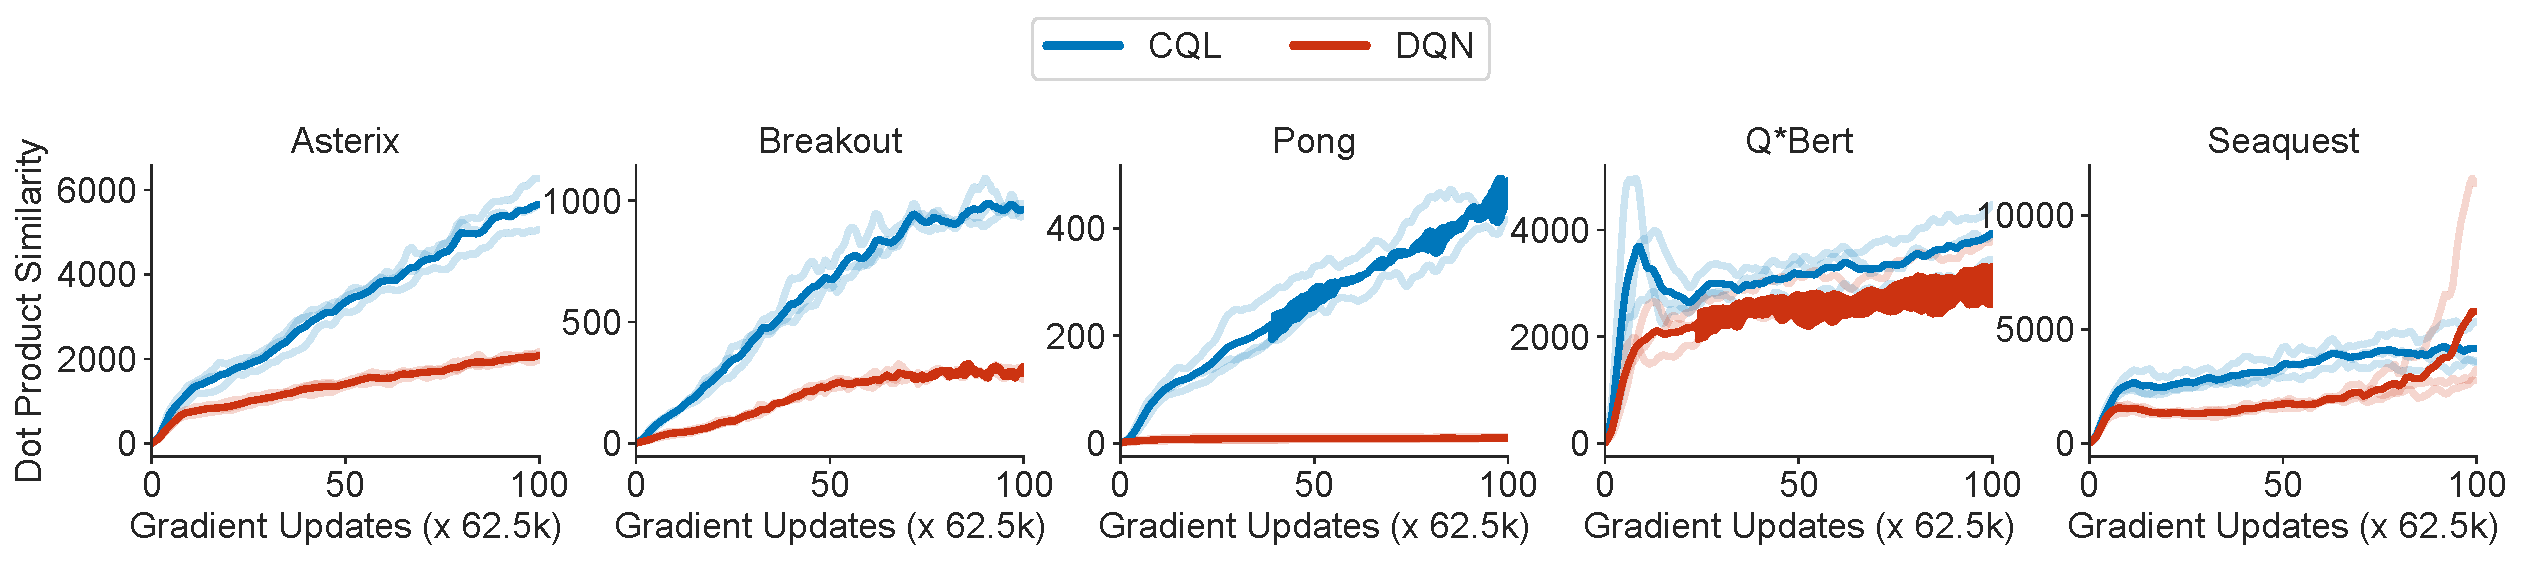
\includegraphics[width=0.99\textwidth]{figures_iclr/figure1_dotproduct_value.pdf}
    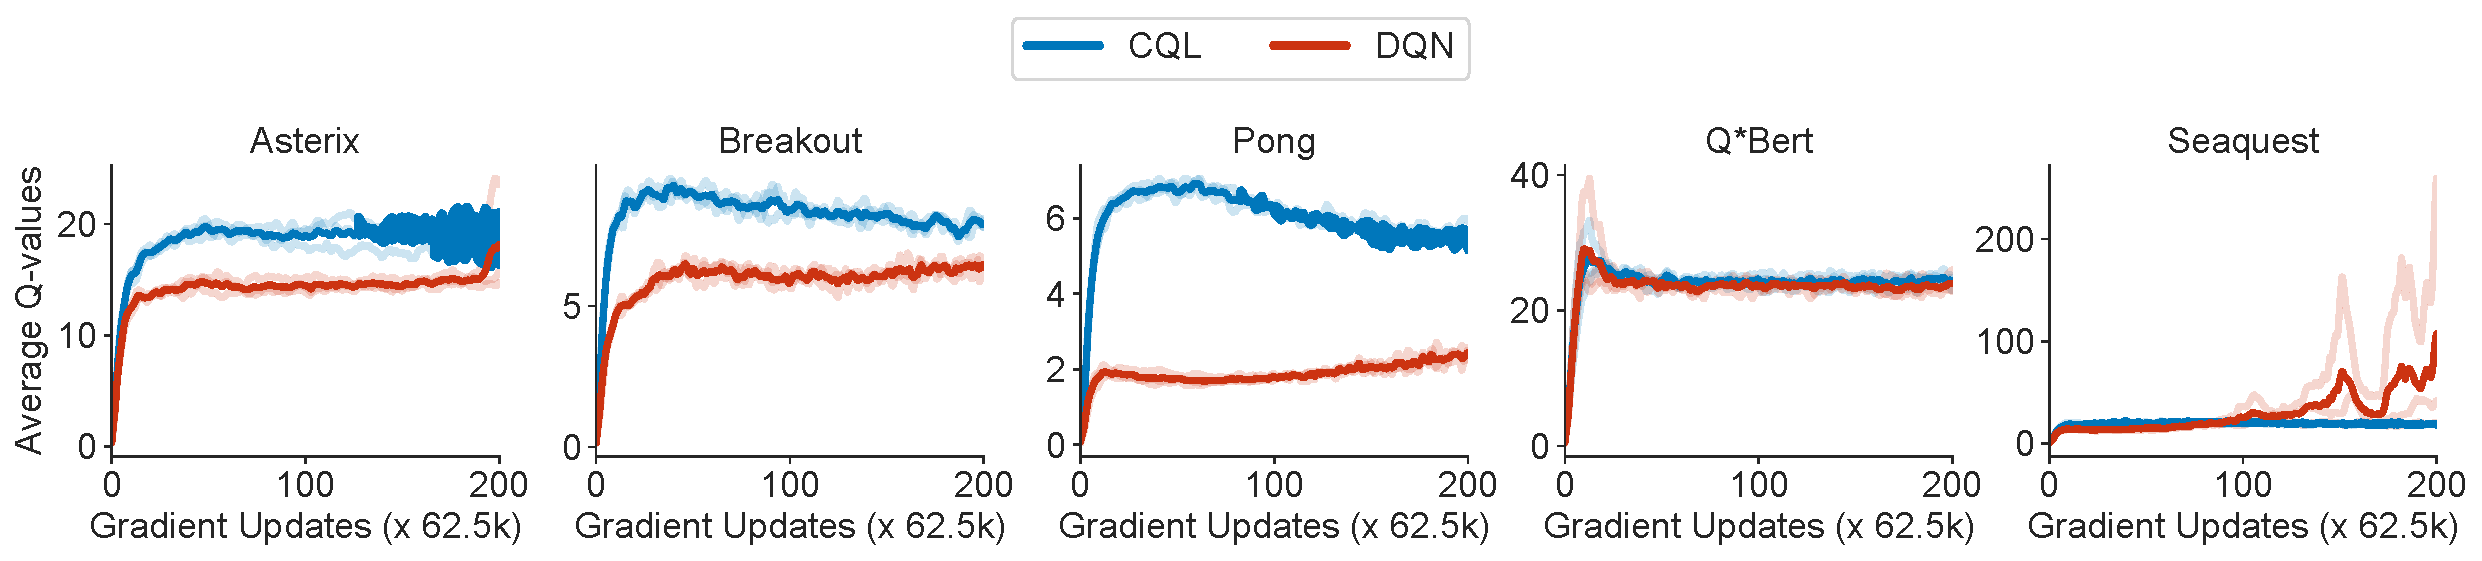
\includegraphics[width=0.99\textwidth]{figures_iclr/figure1_q_vals.pdf}
    \vspace{-5pt}
    \caption{\footnotesize{\label{fig:dot_product_increases_five_games} \textbf{Demonstrating feature co-adaptation on five Atari games with standard offline DQN and CQL, averaged over 3 seeds.} Observe that the feature dot products continue to rise with more training for both CQL and DQN, indicating the presence of co-adaptation. On the other hand, the average Q-values exhibit a converged trend, except on Seaquest. Further, note that the dot products continue to increase for CQL even though CQL explicitly corrects for out-of-distribution action inputs. }}
    \vspace{-0.1in}
\end{figure}

\vspace{-0.1in}
\subsection{{Layer-wise structure of a Q-network trained with DR3}}
\label{app:layerwise}
\vspace{-0.05in}
To understand if DR3 indeed makes Q-networks behave as if they were trained via supervised learning, utilizing the empirical analysis tools from \citet{zhang2019all}, we test the robustness/sensitivity of each layer in the learned network to re-initialization, while keeping the other layers fixed. This tests if a particular layer is \emph{critical} to the predictions of the learned neural network and enables us to reason about generalization properties~\citep{zhang2019all,chatterji2019intriguing}. We ran CQL and REM and saved all the intermediate checkpoints. Then, as shown in Figure~\ref{fig:robustness}, we first loaded a checkpoint ($x$-axis), and computed policy performance (shaded color; colorbar)  by re-initializing a given layer ($y$-axis) of the network to its initialization value before training for the same run.

\begin{figure}[h]
    \centering
    % \begin{subfigure}[c]
    %     \centering
    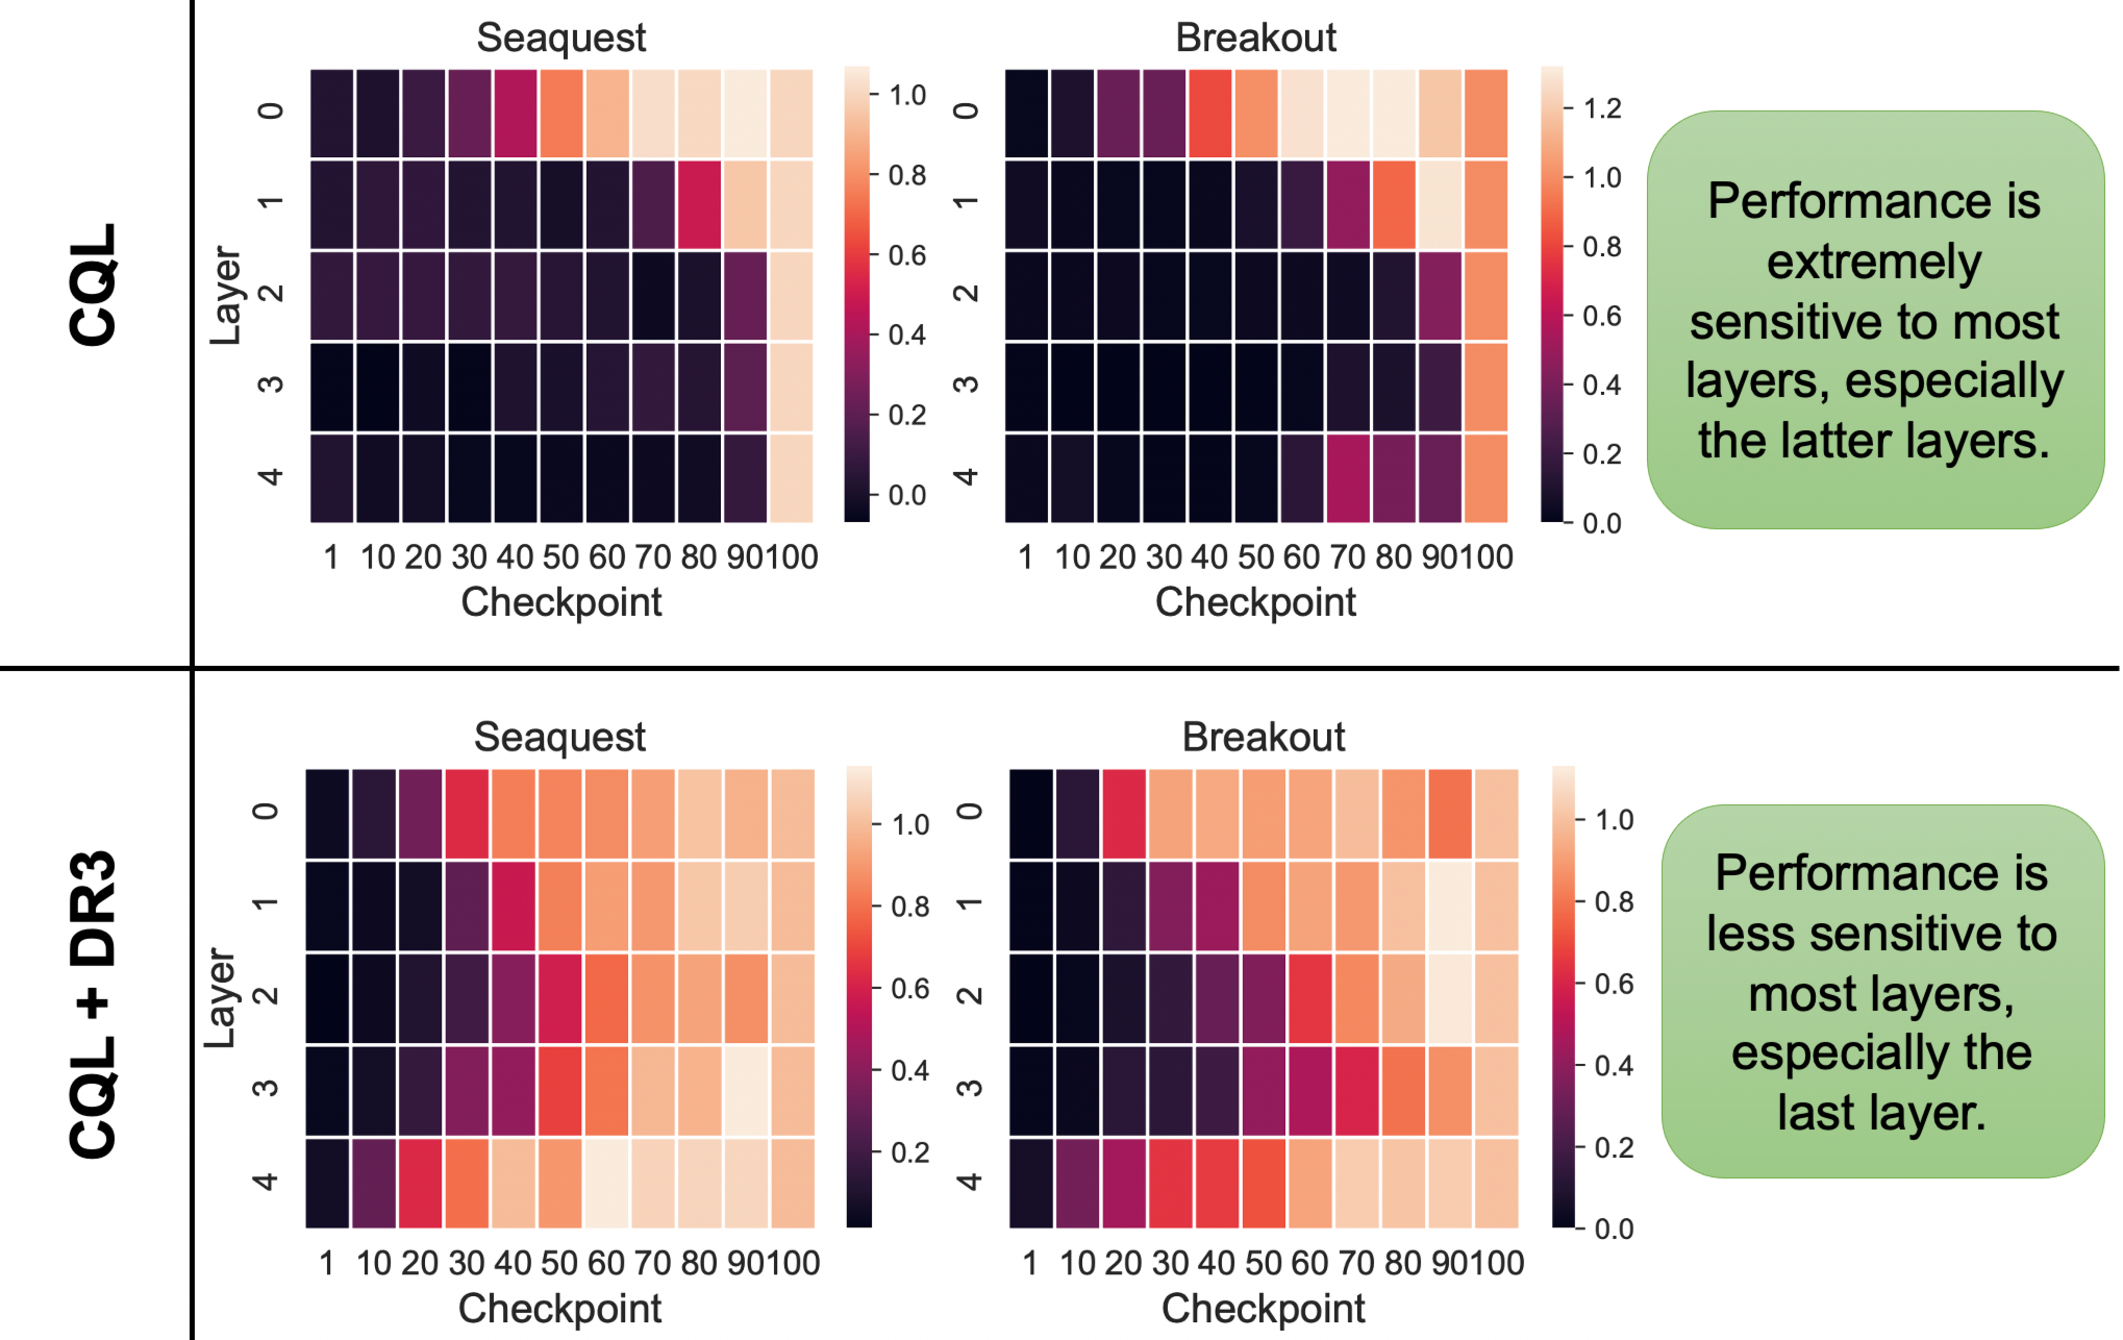
\includegraphics[width=0.612\textwidth]{figures/robustness_figures/layer_robustness_cql.pdf}
    % ~\hline~
    \vspace{0.4cm}
    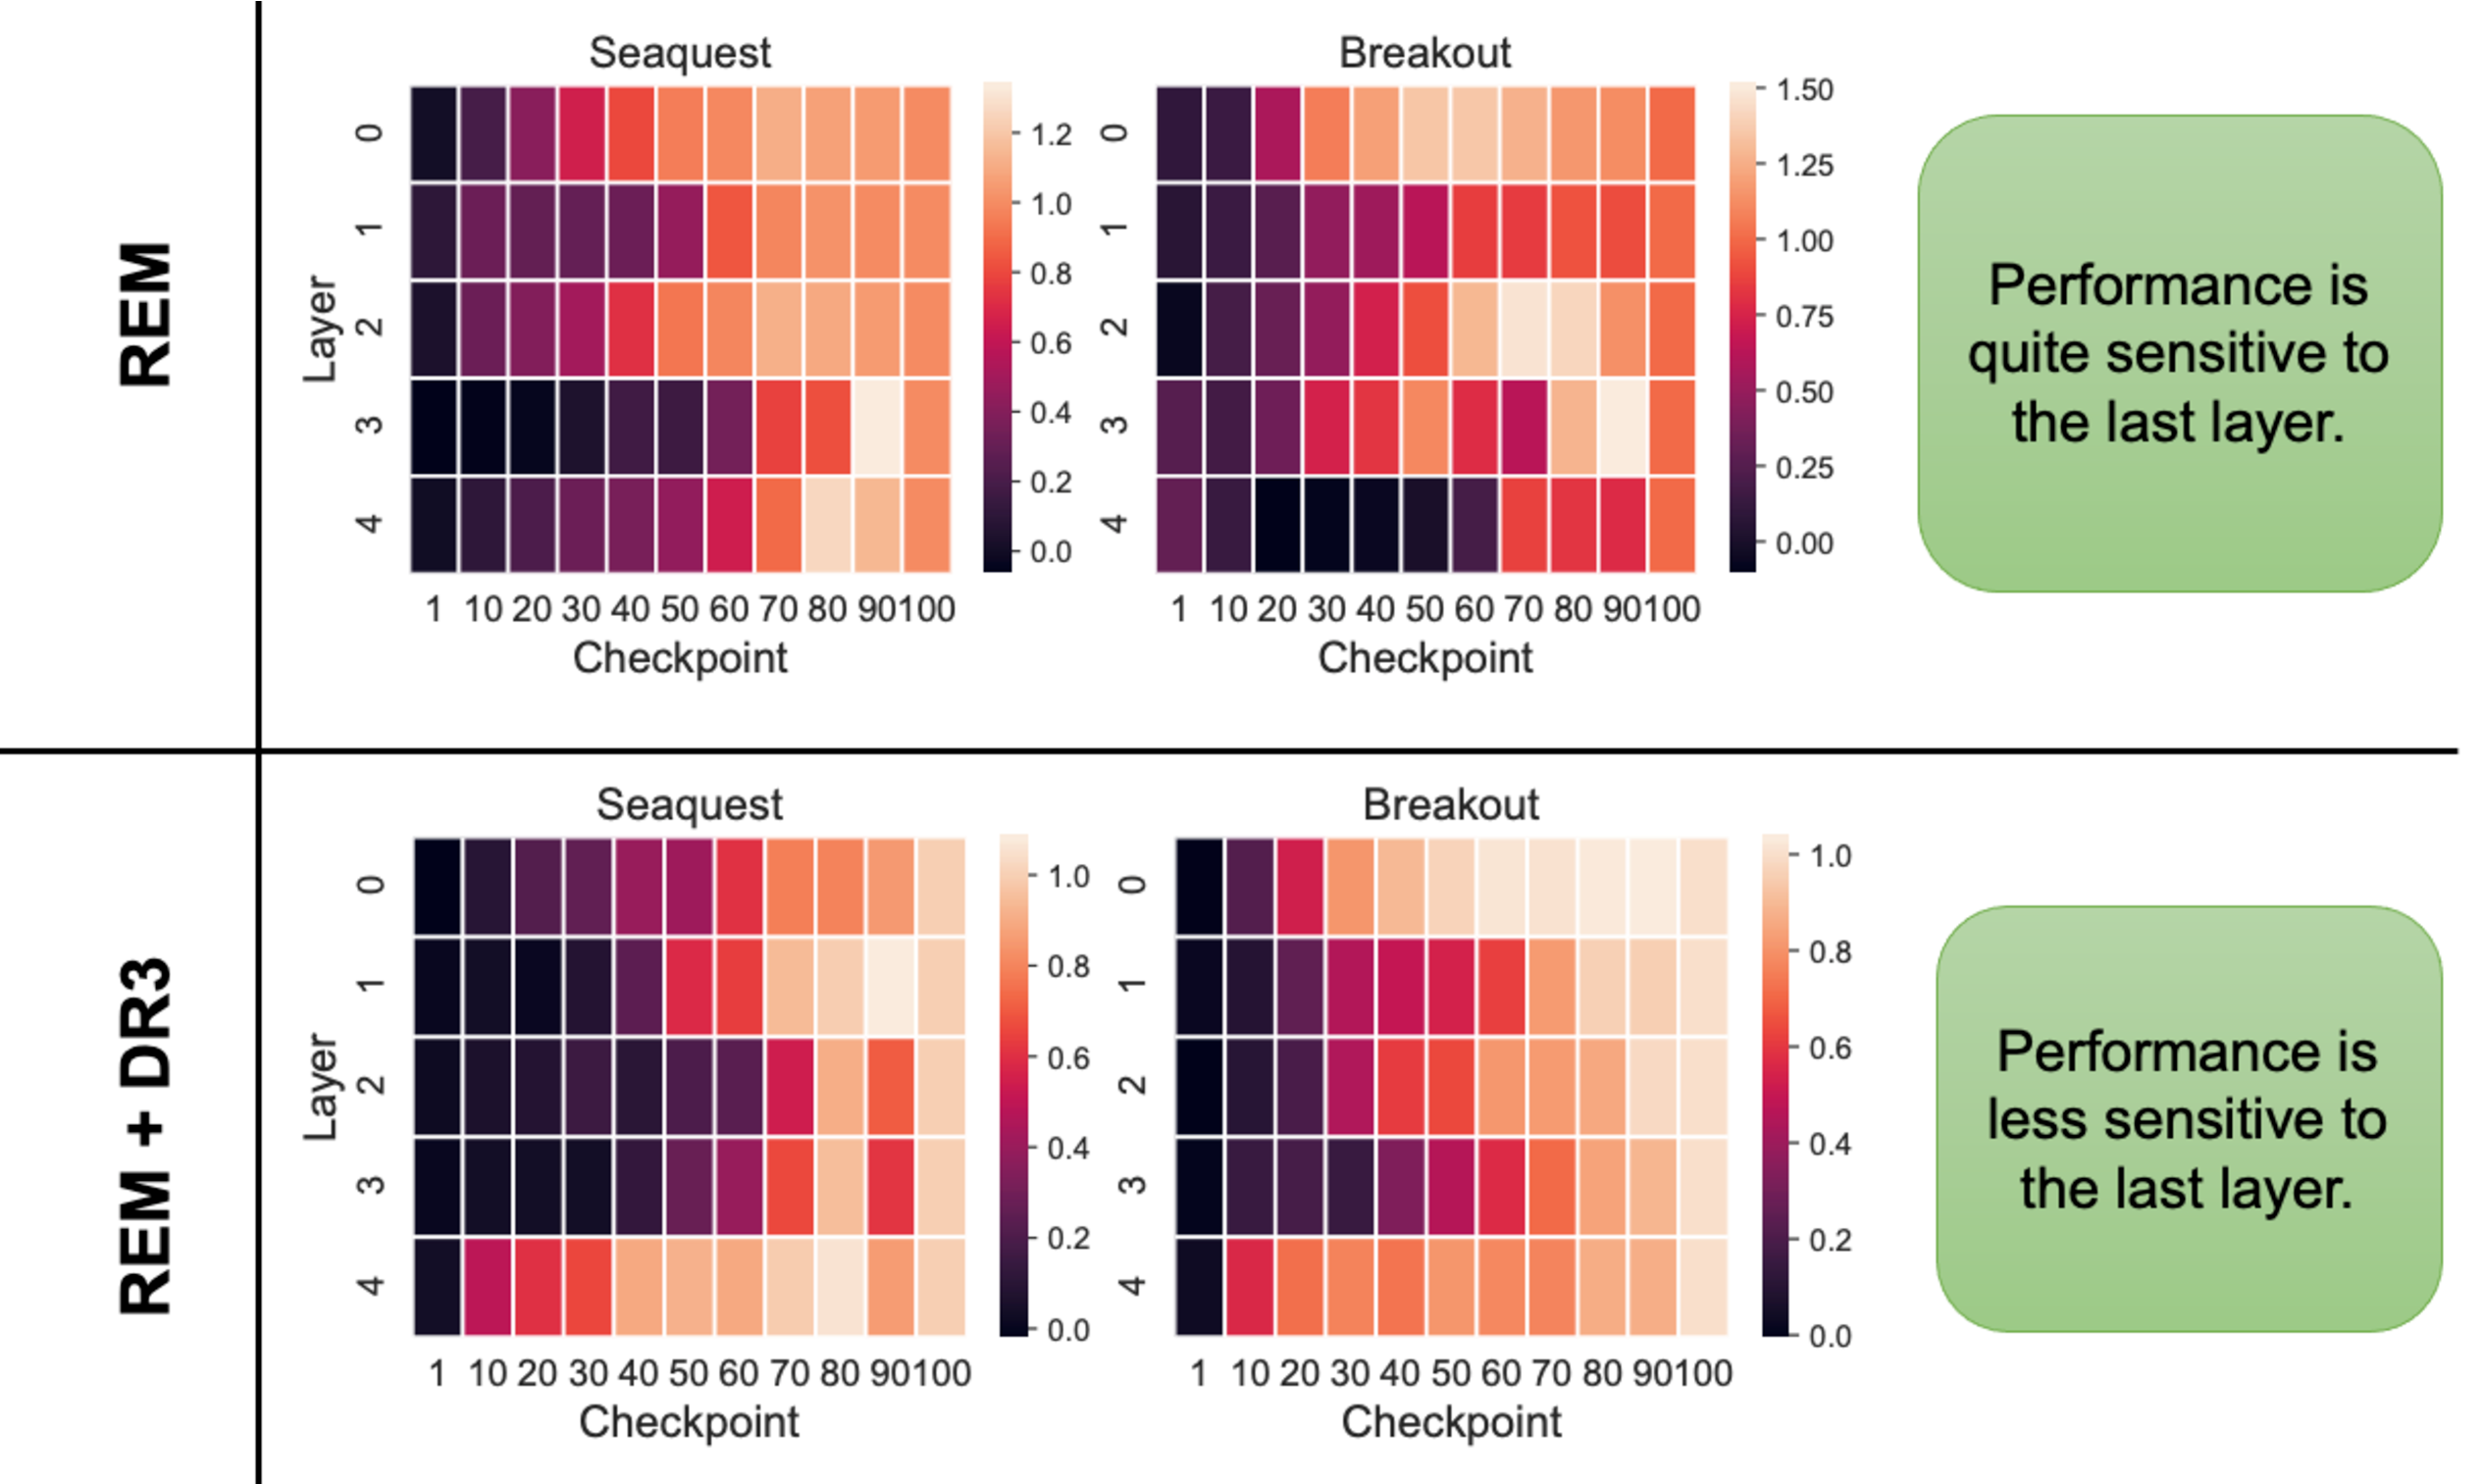
\includegraphics[width=0.622\textwidth]{figures/robustness_figures/rem_robustness_final.pdf}
    \vspace{-5pt}
    \caption{\footnotesize{\label{fig:robustness} \textbf{CQL vs CQL + DR3 and REM vs REM + DR3.} Average robustness of the learned Q-function to re-initialization of all layers to different checkpoints over the course of training created based on the protocol from \citet{zhang2019all}. The colors in the heatmap indicate performance of the reinitialized checkpoint, normalized w.r.t. the checkpoint without any change to layers. Note that while CQL and REM are more sensitive (i.e., less robust) to reinitialization of all the layers especially the last layer, CQL + DR3 and REM + DR3 behave closer to supervised learning, in the sense that they are more robust to reinitialization of layers of the network, especially the last layer.}}
    % \end{subfigure}
    % \caption{\textbf{REM vs REM + \methodname}. Average re-initialization robustness to different checkpoints of all layers for REM~(left) and REM + \methodname~(right). A score of 1 corresponds to same performance as the trained checkpoint while a score of 0 correponds to performance of a randomly initialized model. 
    % Following the protocol in \citep{zhang2019all}, ..}
    % % \begin{subfigure}[c]
    %     \centering
    %     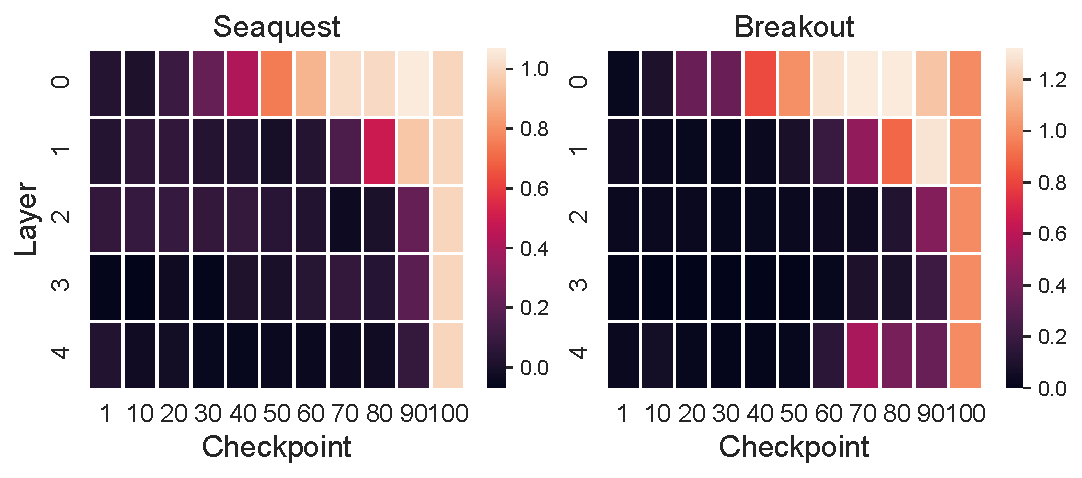
\includegraphics[width=0.47\textwidth]{figures/robustness_figures/cql_robustness.pdf}
    %      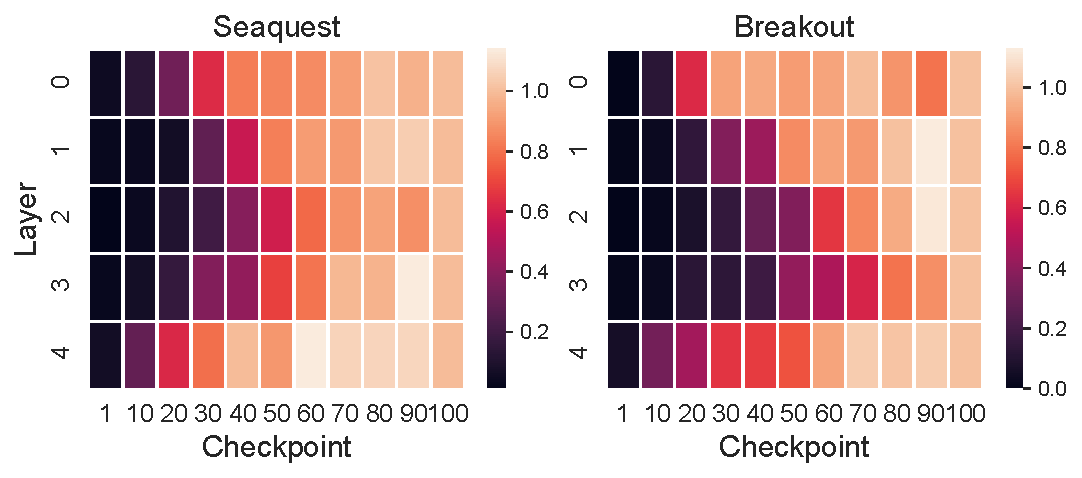
\includegraphics[width=0.47\textwidth]{figures/robustness_figures/dr3_cql_robustness.pdf}
    %      \vspace{-10pt}
    %     \caption{CQL vs CQL + \methodname}
    % % \end{subfigure}
    \vspace{-0.3cm}
\end{figure}
Note in Figure~\ref{fig:robustness}, that while almost all layers are absolutely critical for the base CQL algorithm, 
% and most layers, including the last layer are critical for the REM algorithm~(see \figref{}), 
utilizing DR3 substantially reduces sensitivity to the latter layers in the Q-network over the course of training. This is similar to what \citet{zhang2019all} observed for supervised learning, where the initial layers of a network were the most critical, and the latter layers primarily performed near-random transformations without affecting the performance of the network. This indicates that utilizing DR3 alters the internal layers of a Q-network trained with TD to behave closer to supervised learning.


\vspace{-0.15cm}
\subsection{\rebuttal{Results on MuJoCo Domains}}
\label{app:mujoco}
\rebuttal{In this section, we provide the results of applying DR3 on the MuJoCo tasks shown in Figure A.5. (Appendix A) of \citet{kumar2021implicit}. To briefly describe the setup, in these tasks we train on the three gym tasks (Hopper-v2, Ant-v2, Walker2d-v2) using 20\% of the offline data, uniformly subsampled from the run of an online SAC agent, mimicking the setup from \citet{kumar2021implicit}. Rather than retraining an SAC agent to collect data, we subsampled the Gym-MuJoCo \texttt{*-full-replay-v2} replay buffers from the latest D4RL~\citep{fu2020d4rl}. In these cases we plot the $\mathrm{srank}_\delta$ values, the feature dot products and the corresponding performance values with and without the DR3 regularizer for 4M steps (\citet{kumar2021implicit} showed their plots for just under 4M steps) in Figure~\ref{fig:mujoco_results_from_iup}.}

\begin{figure}[t]
    \centering
    \vspace{-5pt}
    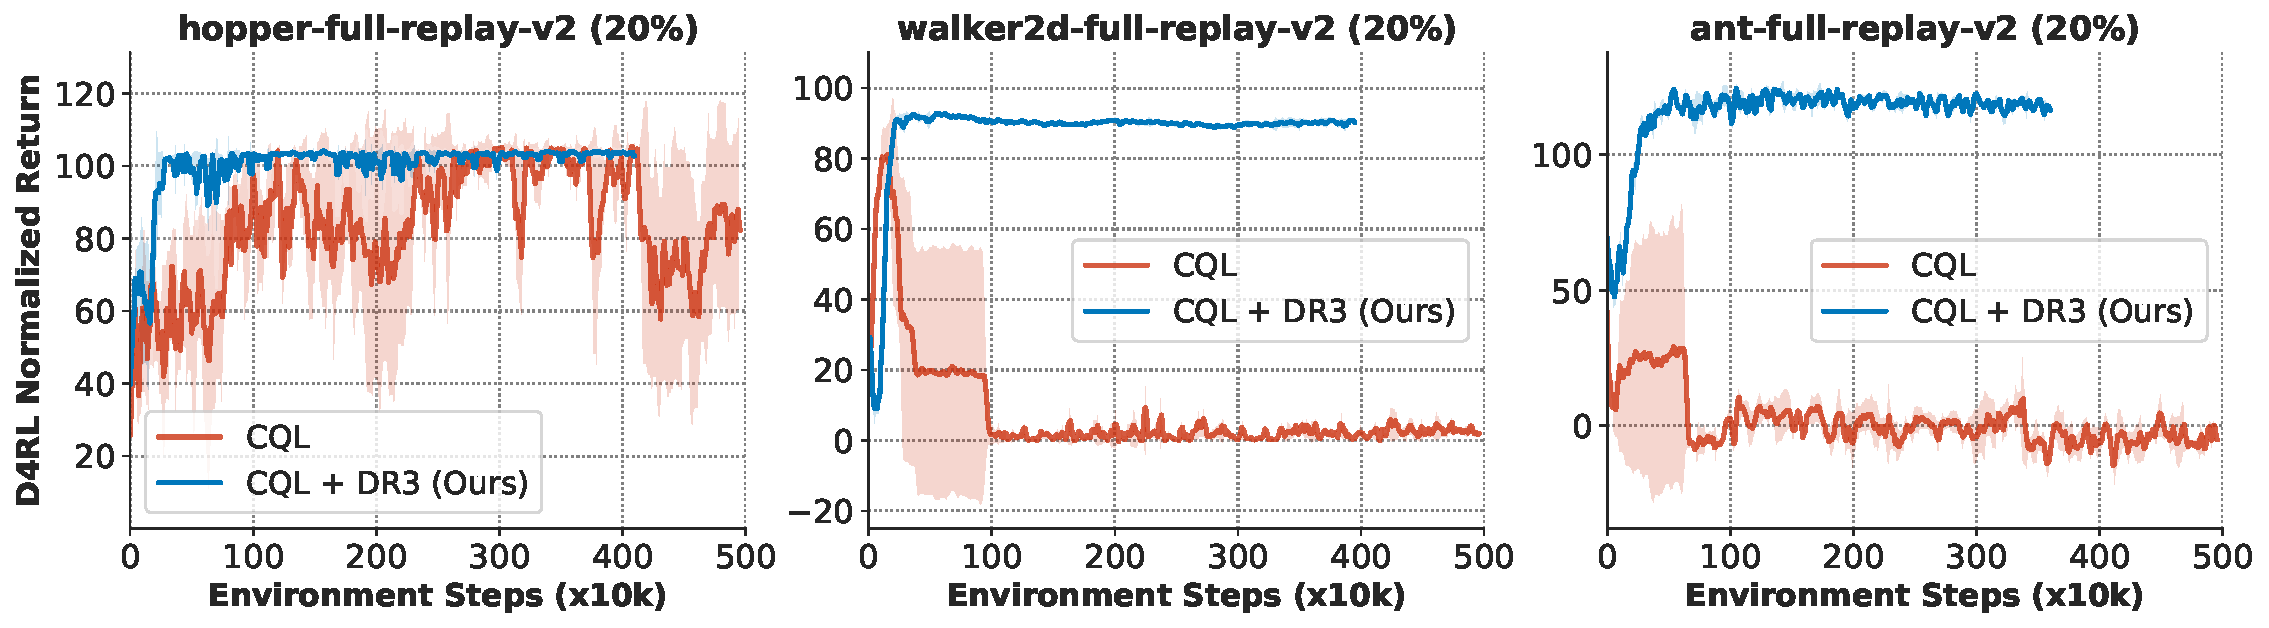
\includegraphics[width=0.89\textwidth]{rebuttal/offline_dr3_mujoco_envs_rebuttal.pdf.pdf}
    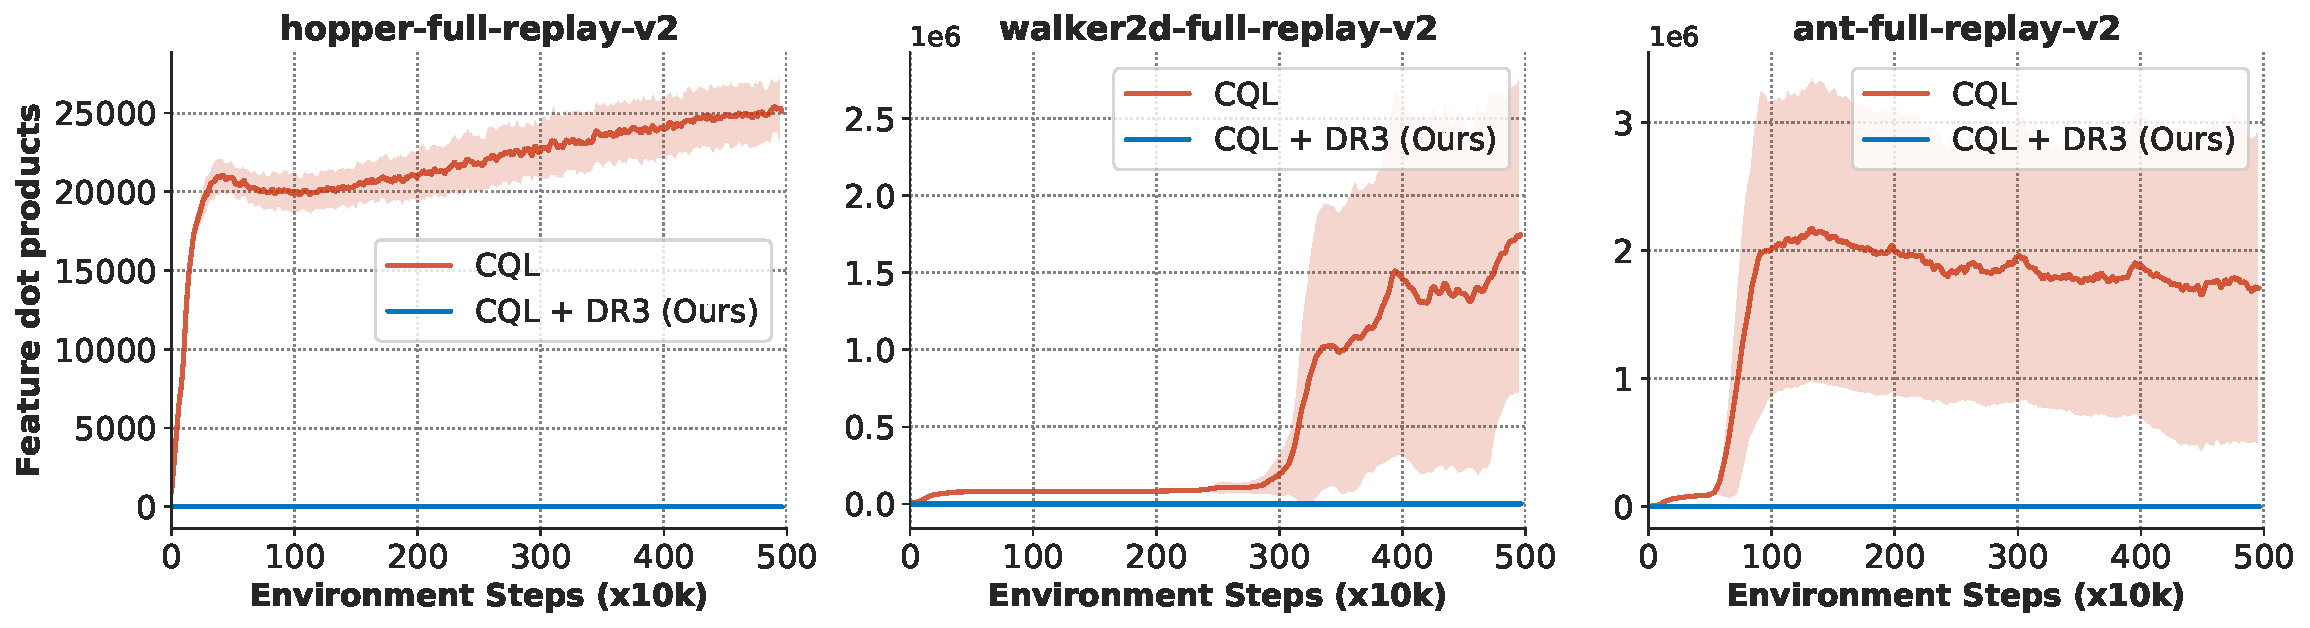
\includegraphics[width=0.89\textwidth]{rebuttal/offline_dr3_mujoco_envs_rebuttal_feat_dot.pdf_final.pdf}
    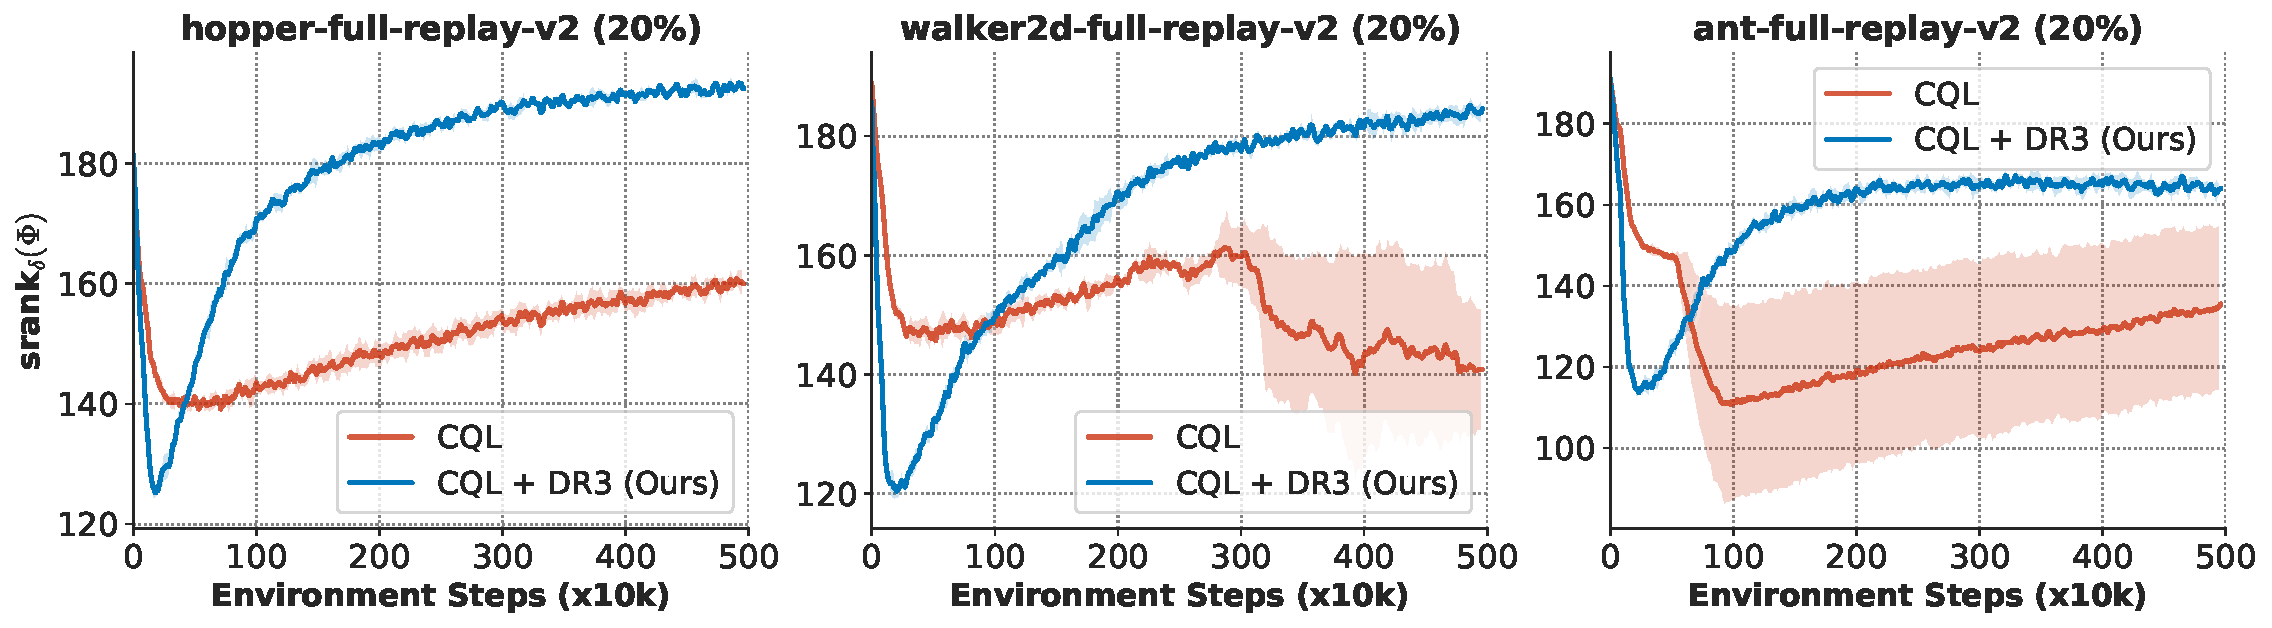
\includegraphics[width=0.89\textwidth]{rebuttal/offline_dr3_mujoco_envs_rebuttal_ranks.pdf.pdf}
    \vspace{-5pt}
    \caption{\footnotesize{\label{fig:mujoco_results_from_iup} \rebuttal{\textbf{Comparison of CQL and CQL + DR3 on the offline MuJoCo Gym domains}, mimicking the setup of \citet{kumar2021implicit}. The data is generated by randomly sampling 20\% of the transitions of the D4RL~\citep{fu2020d4rl} full-replay-v2 datasets, which are collected via the run of an online SAC agent. The performance is shown in terms of the D4RL normalized score, where 0.0 denotes the performance of a random policy and 100.0 denotes the performance of an expert online SAC policy. Observe that adding DR3 stabilizes the performance on Hopper, and prevents performance collapse on Walker2d and Ant. In addition note that the srank values attained by CQL + DR3 is higher than base CQL and more importantly, the feature dot products are much smaller for CQL + DR3 compared to CQL.}}}
    \vspace{-0.1cm}
\end{figure}

\rebuttal{Observe in Figure~\ref{fig:mujoco_results_from_iup}, that while the standard CQL algorithm performs poorly and suffers from performance degradation within about 1M-1.5M steps for Walker2d and Ant, CQL + DR3 is able to prevent the performance degradation and trains stably. Base CQL demonstrates oscillatory performance on Hopper, but CQL + DR3 stabilizes the performace of CQL. This indicates that DR3 is effective on MuJoCo domains, and prevents the instabilities with CQL.}

\rebuttal{For details, the weight on the CQL regularizer in this case is equal to 5.0 across all the tasks, and weight on the DR3 regularizer is 0.01. We also attempted to tune the CQL coefficient for the baseline CQL algorithm within $\{1.0, 2.0, 5.0, 10.0, 20.0\}$ to see if it address the performance degradation issues, but did not find any difference in the collapsing behavior of base CQL. Our CQL baseline is therefore well-tuned, and DR3 improves the performance over this baseline.}

\subsection{Rank Collapse is Alleviated With DR3}
\label{app:rank_collapse_is_gone}

\begin{figure}[h]
    \centering
    % \vspace{-5pt}
    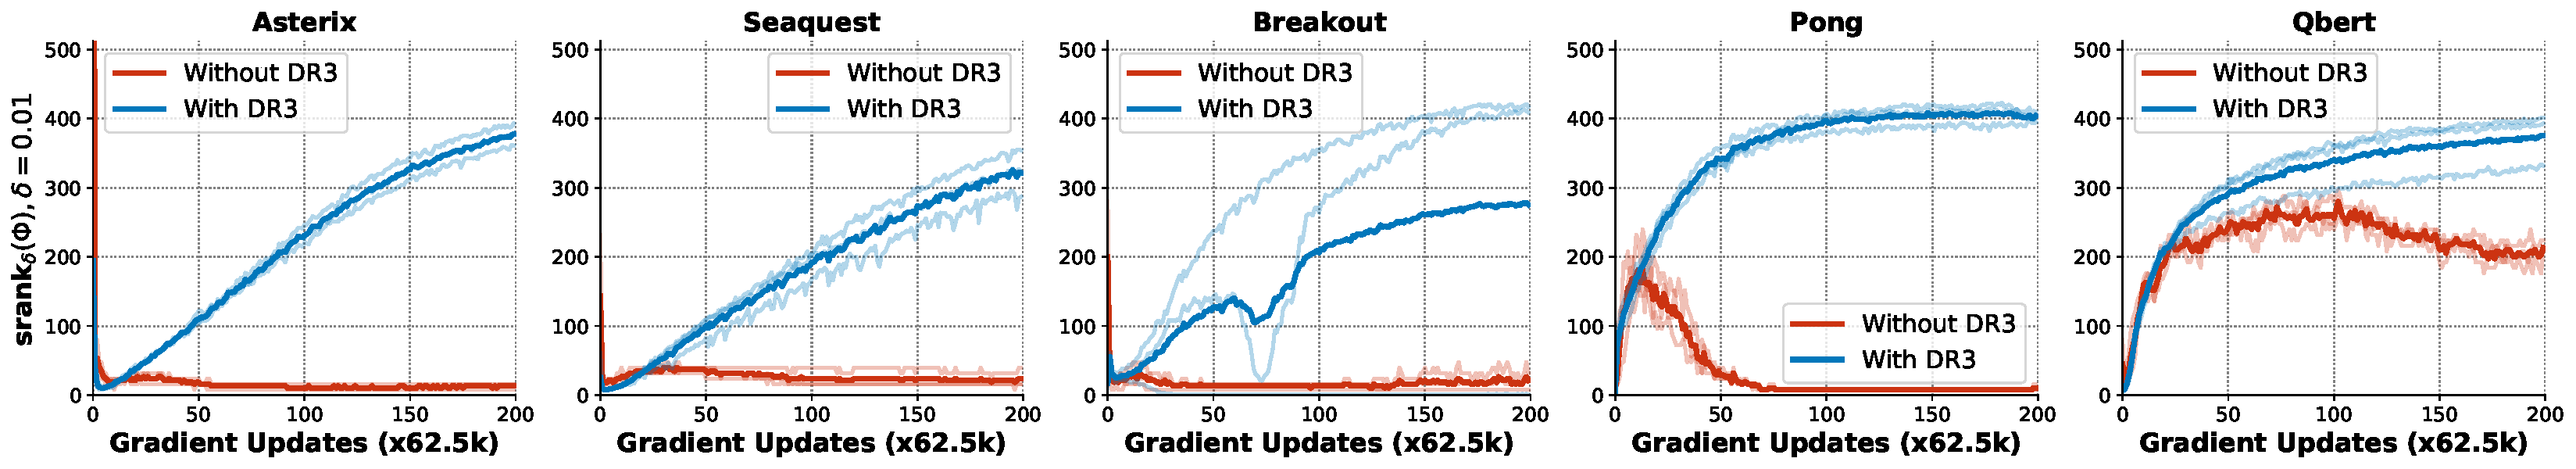
\includegraphics[width=0.99\textwidth]{figures_iclr/rank_trends_dr3_cql.pdf}
    \vspace{-5pt}
    \caption{\footnotesize{\label{fig:rank_trends_5_games} \textbf{Comparing the feature ranks for CQL and CQL + DR3.} Observe that utilizing DR3 successfully alleviates the rank collapse issue noted in prior work without explicitly correcting for it.}}
    % \vspace{-0.5cm}
\end{figure}
Prior work~\citep{kumar2021implicit} has shown that implicit regularization in TD-learning can lead to a feature rank collapse phenomenon in the Q-function, which hinders the Q-function from using its full representational capacity. Such a phenomenon is absent in supervised learning, where the feature rank does not collapse. Since DR3 is inspired by mitigating the effects of the term in the implicit regularizer (Equation~\ref{eqn:regularizer}) that only appears in the case of TD-learning, we wish to understand if utilizing DR3 also alleviates rank collapse. To do so, we compute the effective rank $\mathrm{srank}_\delta(\phi)$ metric of the features learned by Q-functions trained via CQL and CQL with DR3 explicit regularizer. As shown in Figure~\ref{fig:rank_trends_5_games}, for the case of five Atari games, utilizing DR3 alleviates the rank collapse issue completely \rebuttal{(i.e., the ranks do not collapse to very small values when CQL + DR3 is trained for long). We do not claim that the ranks with DR3 are necessarily higher, and infact as we show below, a higher srank of features may not always imply a better solution.} The fact that DR3 can prevent rank collapse is potentially surprising, because no term in the practical DR3 regularizer explicitly aims to increase rank: feature dot products can be made smaller while retaining low ranks by simply rescaling the feature vectors. But, as we observe, utilizing DR3 enables learning features \rebuttal{that do not exhibit collapsed ranks}, thus \rebuttal{we hypothesize} that correcting for appropriate terms in $\mathrm{R}_\mathrm{TD}(\theta)$ can address some of the previously observed pathologies in TD-learning. 


\begin{figure}[h]
    \centering
    \vspace{-10pt}
    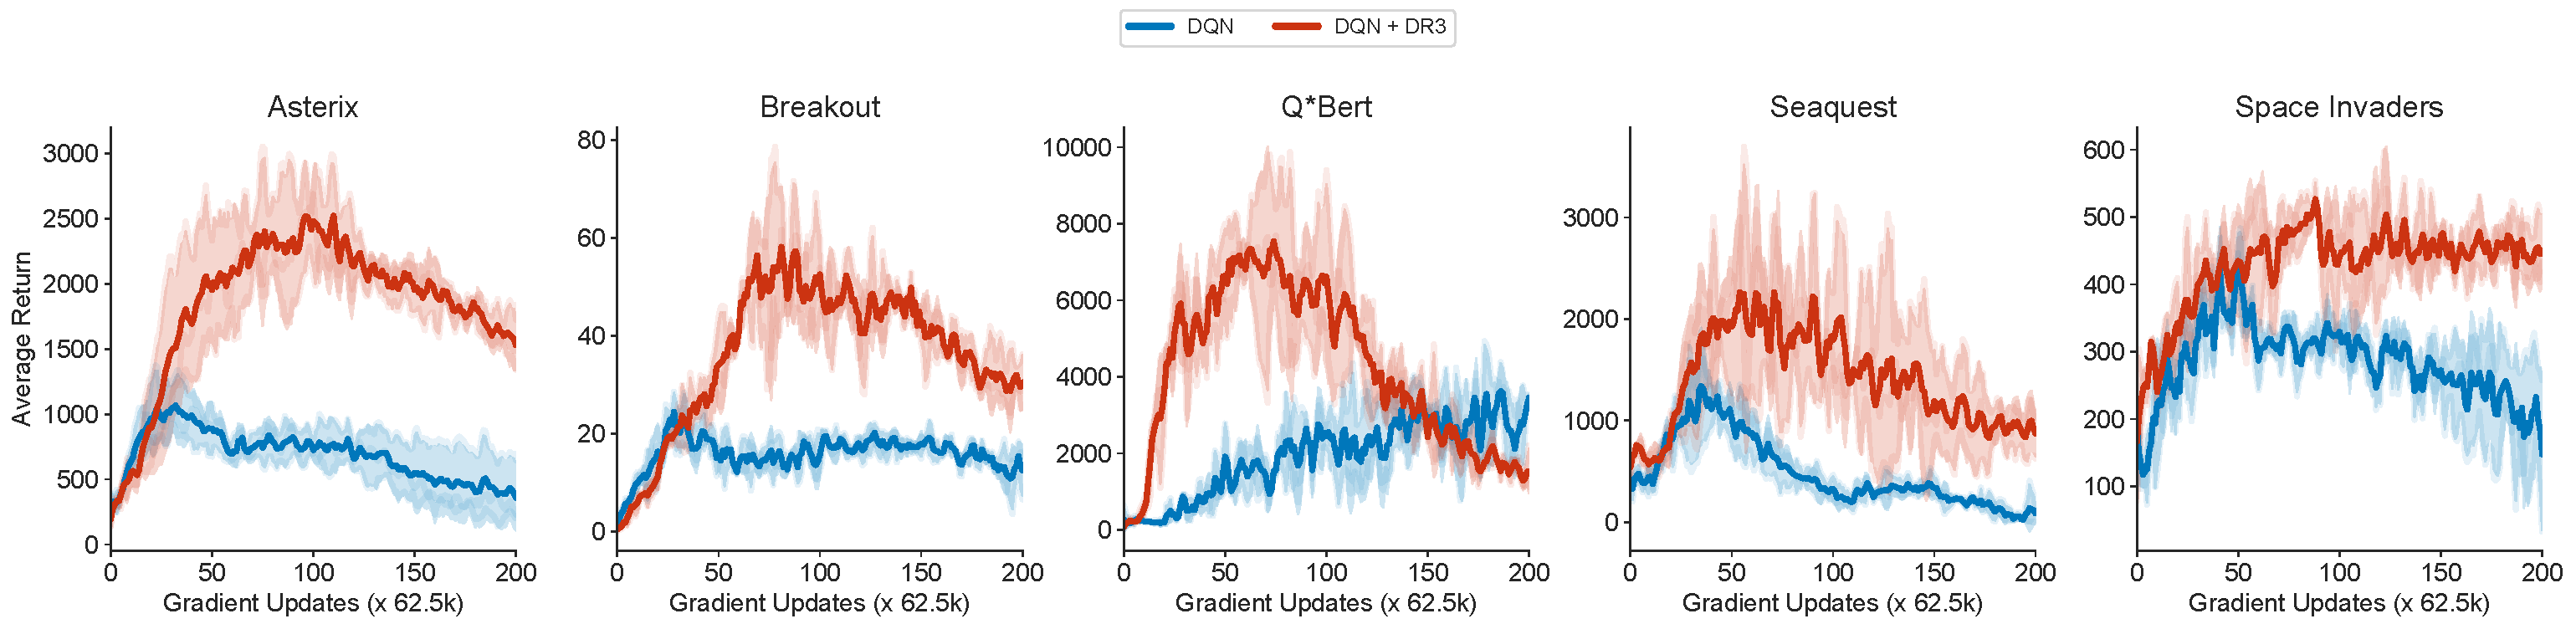
\includegraphics[width=0.99\textwidth]{rebuttal/figure_analysis_dqn_for_rank_collapse_appendix_rebuttal_0.1_final.pdf}
    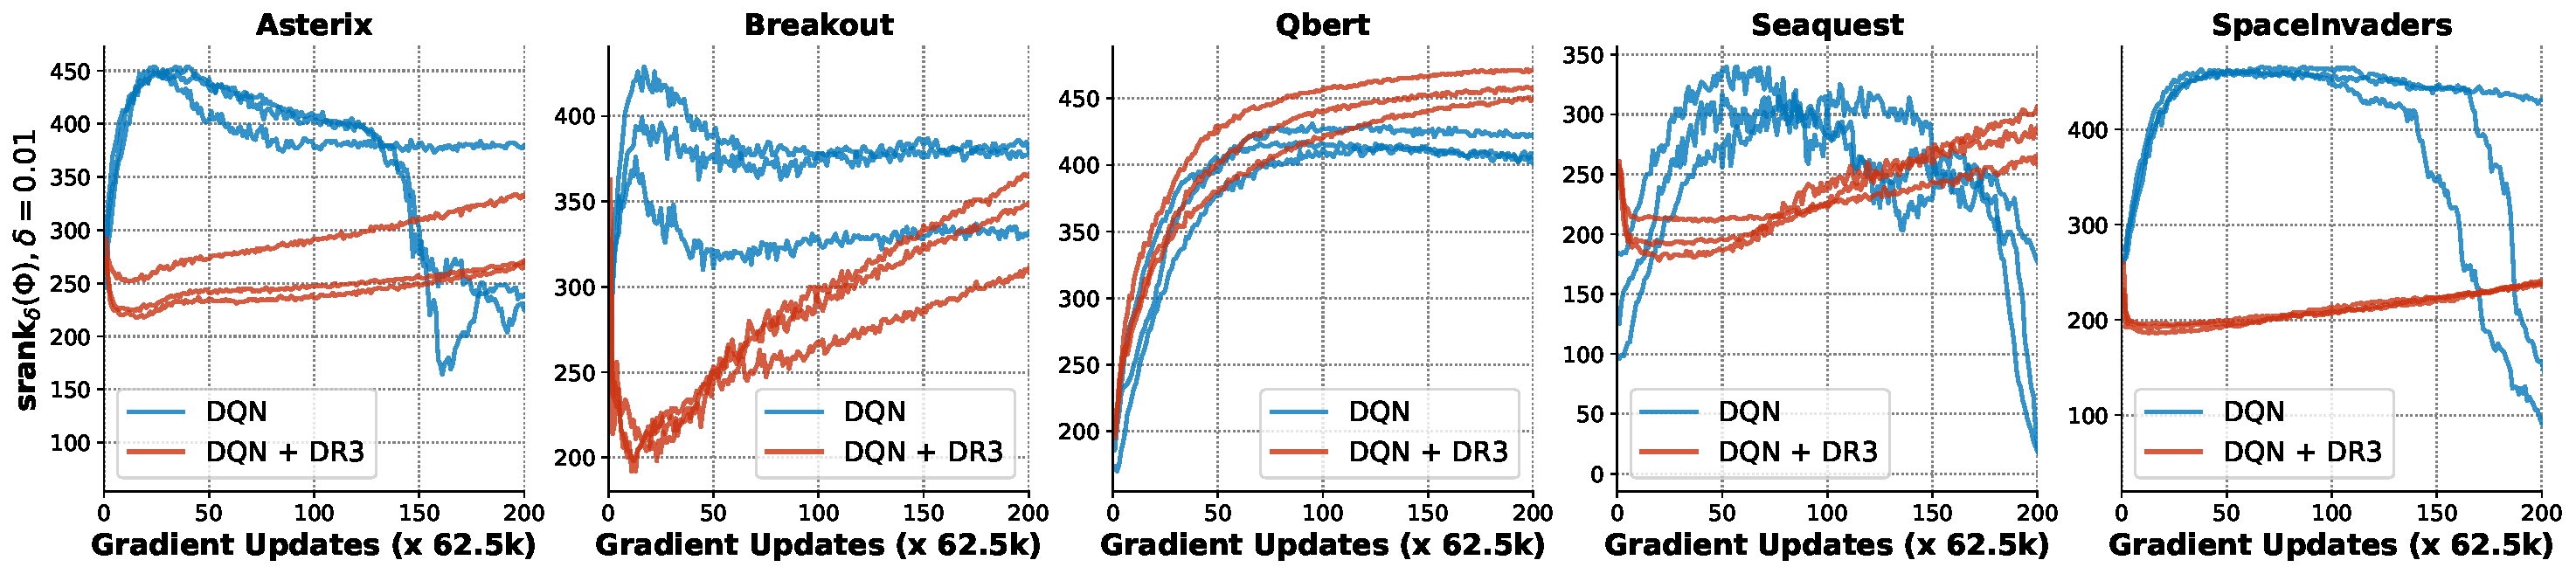
\includegraphics[width=0.99\textwidth]{rebuttal/srank_phi_dqn_rebuttal_200_v4.pdf}
    \vspace{-5pt}
    \caption{\footnotesize{\label{fig:rank_collapse_test_for_dqn} \rebuttal{\textbf{Performance and $\mathrm{srank}$ values for DQN and DQN + DR3.} Observe that the srank values increase for DQN + DR3, while they collapse for DQN on Asterix, Seaquest and SpaceInvaders with more training. Thus, DQN + DR3 does not suffer from a sudden rank collapse. However, a higher srank does not imply a better return, and so while initially DQN does have a high rank, DQN + DR3 performs superiorly.}}}
    \vspace{-0.3cm}
\end{figure}

\rebuttal{We now investigate the feature ranks of a Q-network trained when DR3 is applied in conjunction with a standard DQN and REM~\citep{agarwal2019optimistic} on the Atari domains. We plot the values of $\mathrm{srank}_\delta(\phi)$, the feature dot products and the performance of the algorithm for DQN in Figure~\ref{fig:rank_collapse_test_for_dqn} and for REM in Figure~\ref{fig:rank_collapse_test_for_rem}. In the case of DQN, we find that unlike the base DQN algorithm for which feature rank does begin to collapse with more training, the srank for DQN + DR3 is increasing. We also note that DQN + DR3 attains a better performance compared to DQN, throughout training. }

\begin{figure}[h]
    \centering
    \vspace{-5pt}
    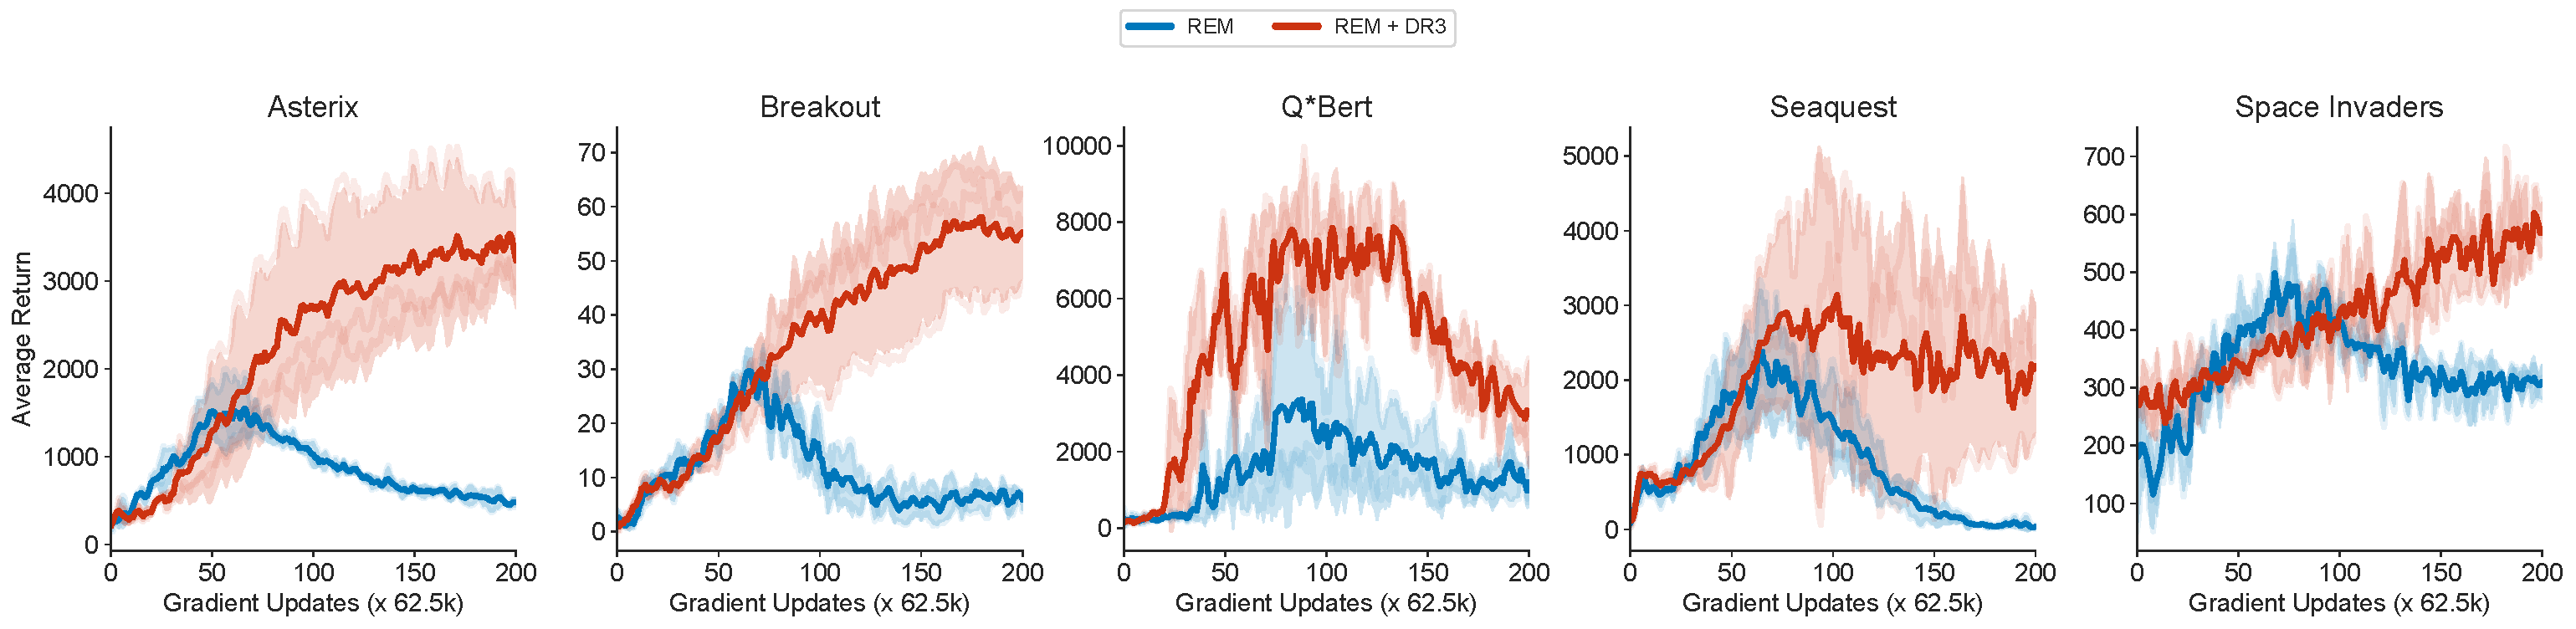
\includegraphics[width=0.99\textwidth]{rebuttal/figure_analysis_rem_for_rank_collapse_appendix_rebuttal_0.001_final.pdf}
    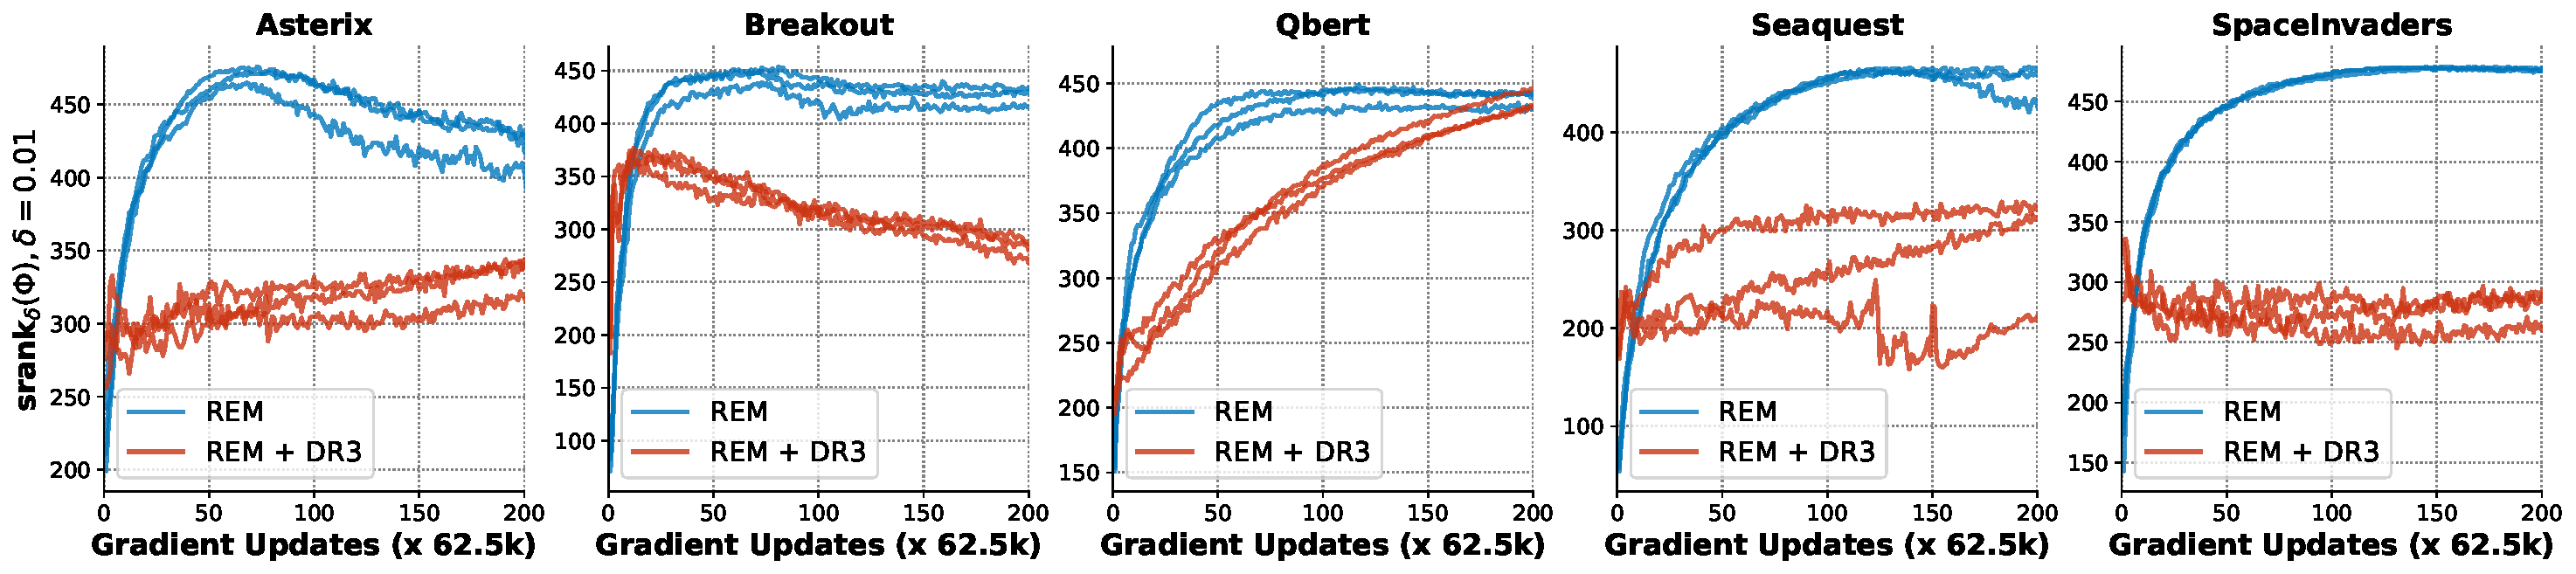
\includegraphics[width=0.99\textwidth]{rebuttal/srank_phi_rem_rebuttal_final_200_v4.pdf}
    \vspace{-5pt}
    \caption{\footnotesize{\label{fig:rank_collapse_test_for_rem} \rebuttal{\textbf{Comparing the performance and $\mathrm{srank}$ values for REM and REM + DR3.} Observe that while REM + DR3 outperforms REM, the $\mathrm{srank}$ values attained by REM are much larger than REM + DR3, and none of these ranks have collapsed. Thus, while REM + DR3 maintains non-collapsed features, for the case of REM, it reduces the value of $\mathrm{srank}$ and attains better performance. This does not contradict the observations from \citet{kumar2021implicit} as we discuss in the text.}}}
\end{figure}

\rebuttal{However, we note that the opposite trend is true for the case of REM: while REM + DR3 attains a better performance than REM, adding DR3 leads to a reduction in the $\mathrm{srank}$ value compared to base REM. At a first glance, this might seem contradicting \citet{kumar2021implicit}, but this is not the case: to our understanding, \citet{kumar2021implicit} establish a correlation between extremely low rank values (i.e., rank collapse) and poor performance, but this does not mean that all high rank features will lead to good performance. We suspect that since REM trains a multi-headed Q-function with shared features and randomized target values, it is able to preserve high-rank features, but this need not mean that these features are useful. In fact, as shown in Figure~\ref{fig:rem_dot_products}, we find that the base REM algorithm does exhibit feature co-adaptation. This case is an example where the srank metric from \citet{kumar2021implicit} may not indicate poor performance.}  

\begin{figure}[h]
    \centering
    \vspace{-10pt}
    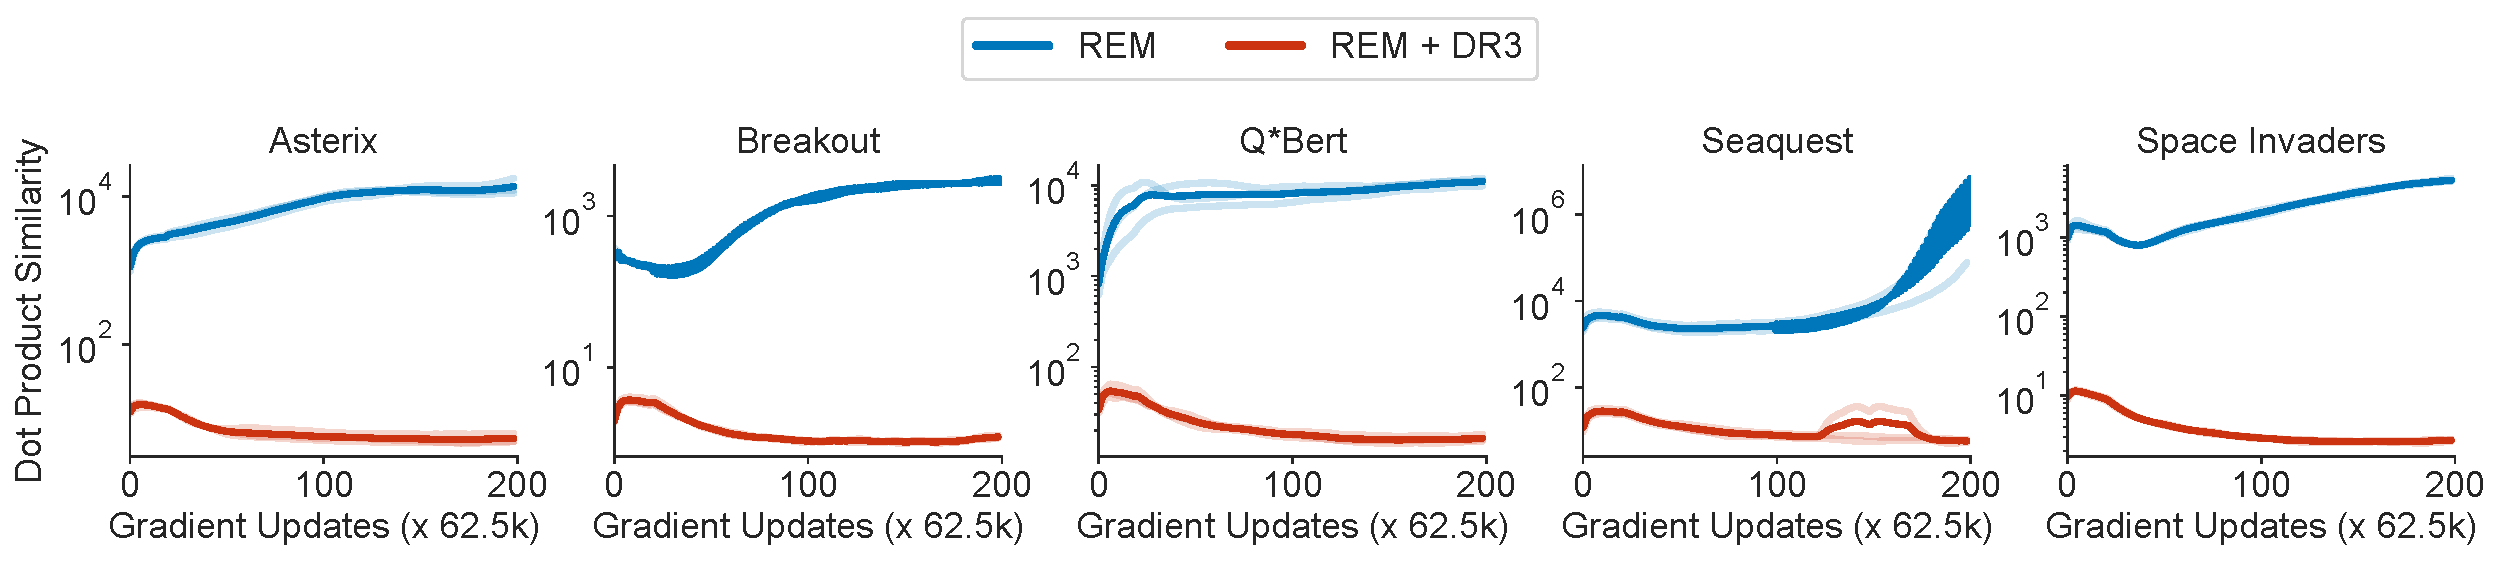
\includegraphics[width=0.99\textwidth]{rebuttal/rebuttal_rem_dotproduct_value_final_v2.pdf}
    \vspace{-5pt}
    \caption{\footnotesize{\label{fig:rem_dot_products} \rebuttal{\textbf{Feature dot products for REM and REM + DR3 on log scale.} REM does suffer from feature co-adaptation despite high-rank features.}}}
    \vspace{-0.3cm}
\end{figure}


\vspace{-0.1cm}
\subsection{Induced Implicit Regularizer: Theory And Practice}
\label{app:theory_practice_gap}
\vspace{-0.1cm}

\begin{table}[t]
    \centering
\fontsize{8}{8}\selectfont
    \centering
    \vspace{-0.05cm}
    \caption{\footnotesize{Normalized interquartile mean performance with 95\% stratified bootstrap CIs~\citep{agarwal2021precipice} across 17 Atari games of REM, REM +  $\Delta'(\Phi)$ (Stop gradient in DR3), REM + \methodname\ after 6.5M gradient steps for the 1\% setting and 12.5M gradient steps for the 5\%, 10\% settings. Observe that REM + $\Delta'(\phi)$ also improves over the base REM method significantly, by about 130\%, even though $\Delta'(\phi)$ is generally comparable and somewhat worse than the DR3 regularizer used in the main paper.}}
    \label{tab:rem_phi_res}
\begin{tabular}{lcccc}
\toprule
% \multirow{2}{*}{\textbf{Data}}  & \multicolumn{4}{c}{\textbf{Stability performance}} \\
Data &  REM & REM + $\Delta'(\Phi)$ & REM+\methodname \\
\midrule
1\%   &  4.0~\ss{(3.3, 4.8)} & 15.0~\ss{(13.4, 16.6)}
& 16.5~\ss{(14.5, 18.6)}  \\
\midrule
5\%   & 25.9~\ss{(23.4, 28.8)} & 55.5~\ss{(50.8, 59.8)} &  60.2~\ss({55.8, 65.1}) \\
\midrule
10\%  & 53.3~\ss{(51.4, 55.3)} & 67.7~\ss{(64.7, 71.3)} & 73.8~\ss{(69.3, 78)} \\
\bottomrule
\vspace{-0.5cm}
\end{tabular}
\end{table}
In this section, we compare the performance of our practical DR3 regularizer to the regularizers (Equation~\ref{eqn:regularizer}) obtained for different choices of $M$, such as $M$ induced by noise, studied in previous work, and also evaluate the effect of dropping the stop gradient function from the practical version of our regularizer.

\textbf{Empirically comparing the explicit regularizers for different noise covariance matrices, $M$.} The theoretically derived regularizer (Equation~\ref{eqn:regularizer}) suggests that for a given choice of $M$, the following equivalent of feature dot products should increase over the course of training: 

\begin{equation}
\label{eqn:general_M}
    \Delta_M(\theta):= \sum_{\bs, \ba \in \mathcal{D}} \mathrm{trace}\left[\Sigma^*_M \nabla Q(\bs, \ba) \nabla Q(\bs', \ba')^\top \right].~~~~~~ \text{(Generalized dot products)}
\end{equation}
We evaluate the efficacy of the explicit regularizer that penalizes the generalized dot products, $\Delta_M(\theta)$, in improving the performance of the policy, \rebuttal{with the goal of identifying if our practical method performs similar to this regularizer on generalized dot products.}. While $\Sigma^*_M$ must be explicitly computed by running fixed point iteration for every parameter iterate $\theta$ found during TD-learning -- which makes this method significantly computationally expensive\footnote{\rebuttal{In our implementation, we run 20 steps of the fixed-point computation of $\Sigma$ as shown in Theorem~\ref{thm:implicit_noise_reg} for each gradient step on the Q-function, and this increases the runtime to about 8 days for 50 iterations on a P100 GPU.}}, we evaluated it on five Atari games for \rebuttal{50 $\times$ 62.5k gradient steps as a proof of concept}. As shown in Figure~\ref{fig:explicit_m_choices}, the DR3 penalty with the choice of $M$ which corresponds to label noise, and the dot product DR3 penalty, which is our main practical approach in this paper generally perform similarly on these domains, attaining almost identical learning curves on \textbf{4/5 games}, and clearly improving over the base algorithm. This hints at the possibility of utilizing other noise covariance matrices to derive an explicit regularizer. \rebuttal{Deriving more computationally efficient versions of the regularizer for a general $M$ and identifying the best choice of $M$ are subject to future work.}

\begin{figure}[t]
    \centering
    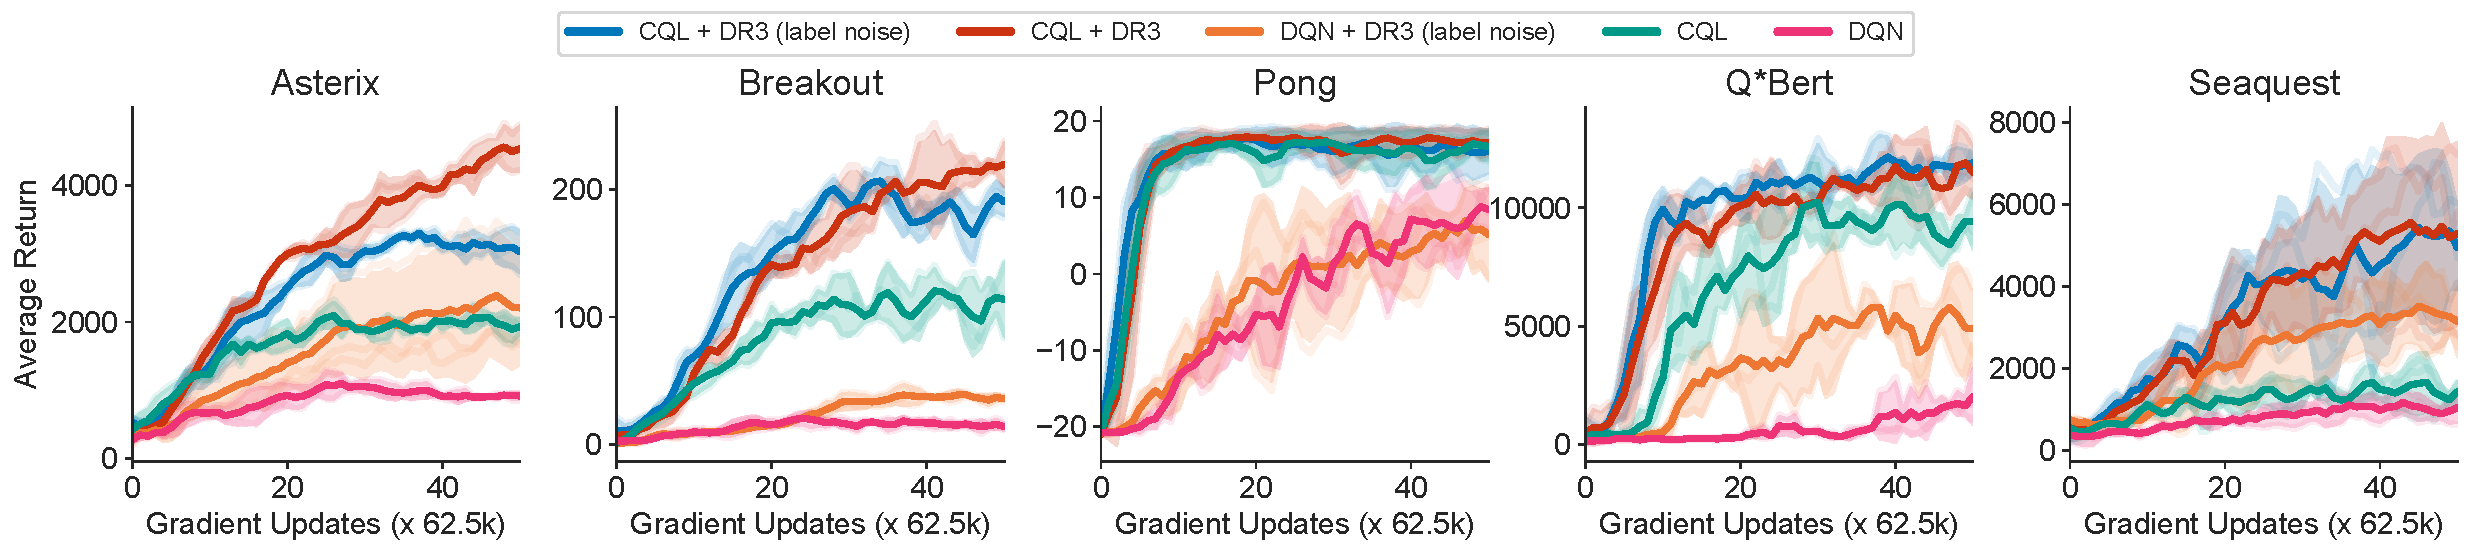
\includegraphics[width=0.99\textwidth]{figures_iclr/figure_analysis_different_dr3_penalty.pdf}
    \vspace{-5pt}
    \caption{\footnotesize{\label{fig:explicit_m_choices} \textbf{Comparing the performance of explicit penalties for two different choices of the covariance matrix $M$.} Observe that in all the five games the DR3 regularizer derived for the choice of $M$ from \citet{blanc2020implicit} also leads to a substantial increase in performance over the base algorithm, and in four of five games, DR3 (label-noise) works just as well as DR3.}}
    \vspace{-0.25cm}
\end{figure}

\textbf{Effect of stop gradient.} Finally, we investigate the effect of utilizing a stop gradient in the DR3 regularizer. We run a variant of DR3: $\Delta'(\phi) = \sum_{\bs, \ba, \bs'} \phi(\bs, \ba)^\top [[\phi(\bs', \ba')]]$, with the stop gradient on the second term $(\bs', \ba')$ and present a comparison to the one without the stop gradient in Table~\ref{tab:rem_phi_res} for REM as the base offline method, averaged over 17 games. Note that this version of DR3, with the stop gradient, also improves upon the baseline offline RL method (i.e., REM) by \textbf{130\%}. While this performs largely similar, but somewhat worse than the complete version without the stop gradient, these results do indicate that utilizing $\Delta'(\phi)$ can also lead to significant gains in performance.


\subsection{\rebuttal{Understanding Feature Co-Adaptation Some More}}
\vspace{-0.2cm}
\rebuttal{In this section, we present some more empirical evidence to understand feature co-adaptation. The three factors we wish to study are: \textbf{(1)} the effect of target update frequency on feature co-adaptation; \textbf{(2)} understand the trend in normalized similarities and compare these to the trend in dot products; and \textbf{(3)} understand the effect of out-on-sample actions in TD-learning and compare it to  offline SARSA on a simpler gridworld domain. We answer these questions one by one via experiments aiming to verify each hypothesis.}

\begin{wrapfigure}{r}{0.6\textwidth}
    \centering
    \vspace{-0.5cm}
    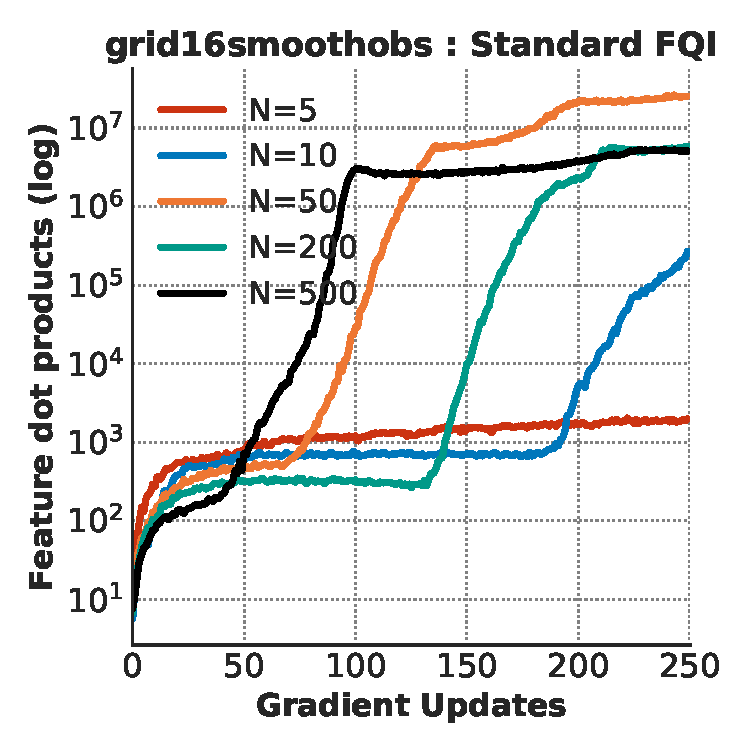
\includegraphics[width=0.47\linewidth]{rebuttal/cql_alpha0_target_delay_coadaptation.pdf}
    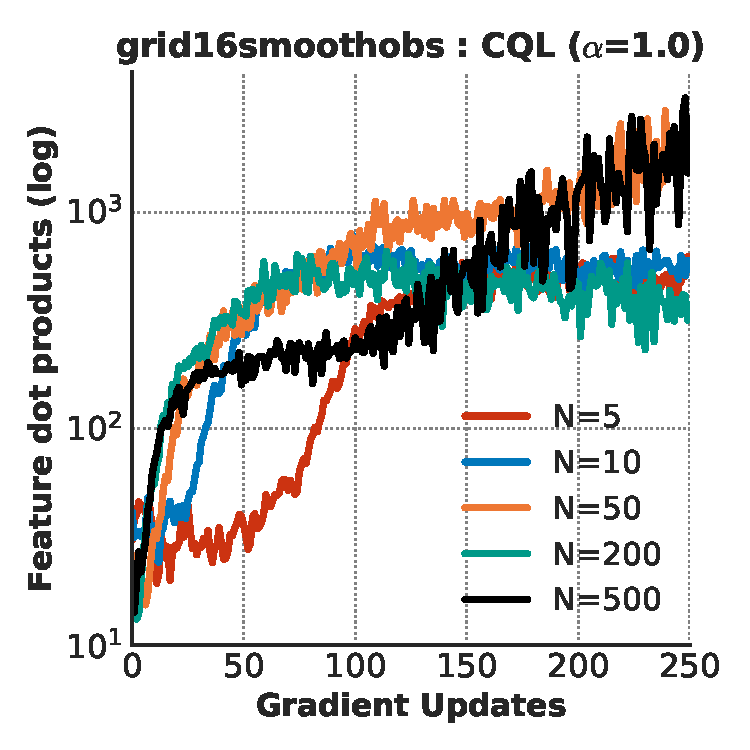
\includegraphics[width=0.47\linewidth]{rebuttal/cql_alpha_1_target_delay_coadaptation.pdf}
    \vspace{-0.3cm}
    \caption{\label{fig:target_update_frequency} \footnotesize{\rebuttal{\textbf{Comparing the feature dot products for various target update delays}, where a smaller $N$ implies a faster update and a larger $N$ corresponds to a slower target update. Observe that while slower updates to the target network may reduce co-adaptation, very slow target updates may still lead to excesssive co-adaptation.}}} 
    % \label{fig:1d_mdp}
    \vspace{-0.6cm}
\end{wrapfigure}
\subsubsection{\rebuttal{Effect of Target Update Frequency on Feature Co-Adaptation}}
\rebuttal{We studied the effect of target update frequency on feature co-adaptation, on some gridworld domains from \citet{fu2019diagnosing}. We utilized the \texttt{grid16smoothobs} environment, where the goal of the agent is to navigate from the center of a $16 \times 16$ gridworld maze to one of its corners while avoiding obstacles and ``lava'' cells. The observations provided to the RL algorithm are given by a high-dimensional random transformation of the $(x, y)$ coordinates, smoothed over neighboring cells in the gridworld. We sampled an offline dataset of 256 transitions and trained a Q-network with two hidden layers of size $(1024, 1024)$ via fitted Q-iteration (FQI)~\citep{Riedmiller2005}.}


\rebuttal{We evaluated the feature dot products for Q-functions trained with a varying target update frequencies, given generically as: updating the target network using a hard target update once per $N$ gradient steps, where $N$ takes on values $N=5, 10, 50, 100, 200, 500$, and present the results in Figure~\ref{fig:target_update_frequency} (left), averaged over 3 random seeds. Thee feature dot products initially decrease from $N=5$ to $N=10$, because the target network is updated slower, but then starts to rapidly increase when when the target network is slowed down further to $N=50$ and $N=200$ in one case and $N=500$ in the other case.} \rebuttal{We also evaluated the feature dot products when using CQL as the base offline RL algorithm. As shown in Figure~\ref{fig:target_update_frequency} (right), while CQL does reduce the absolute range of the feature dot products, slow target updates with $N=500$ still lead to the highest feature dot products as training progresses.}

\rebuttal{\textbf{Takeaway:} While it is intuitive to think that a slower target network might alleviate co-adaptation, we see that this is not the case empirically with both FQI and CQL, suggesting a deeper question that is an interesting avenue for future study.}


\subsubsection{\rebuttal{Gridworld Experiments Comparing TD-learning And Offline SARSA}}
\label{app:exact_behavior_policy}
\rebuttal{To supplement the analysis in Section~\ref{app:problem_more}, we ran some experiments in the gridworld domains from \citet{fu2019diagnosing}. In this case, we used the \texttt{grid16smoothsparse} and \texttt{grid16randomsparse} domains, which present challenging navigation tasks in a maze under a 0-1 sparse reward signal, provided at the end of the trajectory. Additionally, the observations available to the offline RL agent do not consist of the raw $(x, y)$ locations of the agent in the maze, but rather high-dimensional randomly chosen transformations of $(x, y)$ in the case of \texttt{grid16randomsparse}, which are additionally smoothed locally around a particular state to obtain \texttt{grid16smoothsparse}.}

\rebuttal{Since our goal is to compare feature co-adaptation in TD-learning and offline SARSA, we consider a case where we evaluate a ``mixed'' behavior policy that chooses the optimal action with a probability of 0.7 at a given state, and chooses a random, suboptimal action with 0.3. We then generate a dataset of size $256$ transitions and train offline SARSA and TD-learning on this data. While SARSA backups the next action observed in the offline dataset, TD-learning computes a full expectation of the Q-function $\E_{\ba' \sim \pi_\beta(\cdot|\bs')}\left[Q(\bs', \ba')\right]$ under the behavior policy for computing Bellman backup targets. The behavior policy is fully known to the TD-learning agent. Our Q-network consists of two hidden layers of size $(1024, 1024)$ as before.}

\begin{wrapfigure}{r}{0.6\textwidth}
    \centering
    \vspace{-0.5cm}
    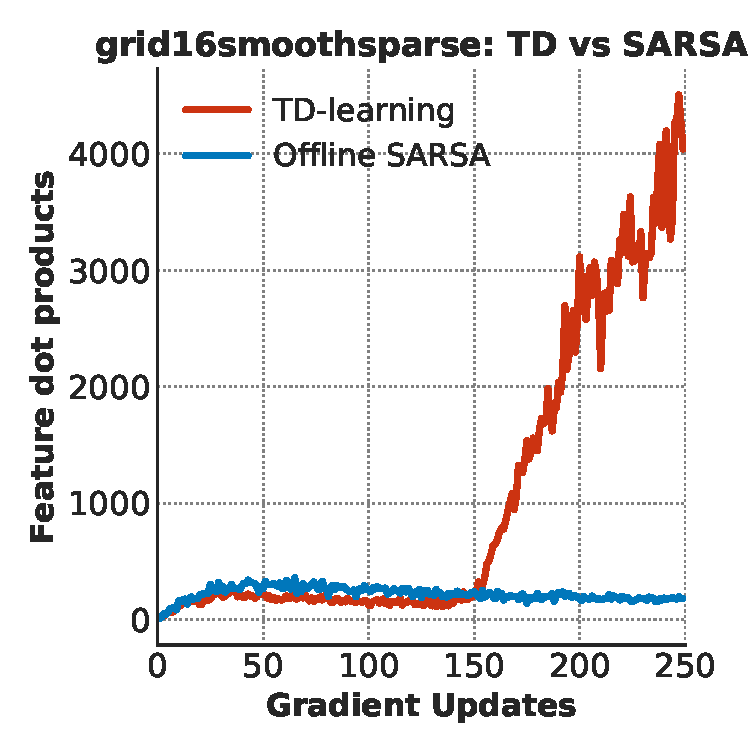
\includegraphics[width=0.47\linewidth]{rebuttal/smoothsparse_td_vs_q.pdf}
    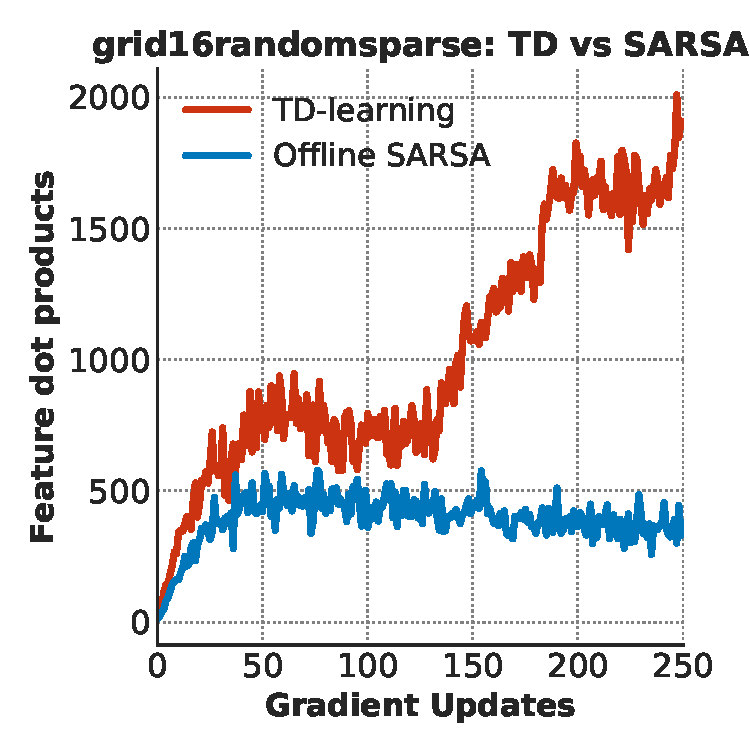
\includegraphics[width=0.47\linewidth]{rebuttal/randomsparse_td_vs_q.pdf}
    \vspace{-0.3cm}
    \caption{\label{fig:out_of_sample_actions} \footnotesize{\rebuttal{\textbf{Comparing the feature dot products for TD-learning and offline SARSA}, used to compute the value of the behavior policy using a dataset of size 256 on two gridworld domains. Observe that the feature dot products are higher in the case of TD-learning compared to offline SARSA.}}} 
    % \label{fig:1d_mdp}
    % \vspace{-0.5cm}
\end{wrapfigure}
\rebuttal{We present the trends in the feature dot products for TD-learning and offline SARSA in Figure~\ref{fig:out_of_sample_actions}, averaged over three seeds. Observe that the trends in the dot product values for TD-learning and offline SARSA closely follow each other for the initial few gradient steps, soon, the dot products in TD-learning start growing faster. In contrast, the dot products for SARSA either saturate or start decreasing. The only difference between TD-learning and SARSA is the set of actions used to compute Bellman targets -- while the actions used for computing Bellman backup targets in SARSA are in-sample actions and are observed in the dataset, the actions used by TD-learning may be out-of-sample, but are still within the distribution of the data-generating behavior policy. This supports our empirical evidence in the main paper showing that out-of-sample actions can lead to feature co-adaptation.}

\subsubsection{\rebuttal{Feature Co-Adaptation and Normalized Feature Similarities}}
\rebuttal{Note that we characterized feature co-adaptation via the dot products of features. In this section, we explore the trends in other notions of similarity, such as cosine similarity between $\phi(\bs, \ba)$ and $\phi(\bs', \ba')$ which measures the dot product of feature vectors at consecutive state-action tuples after normalization. Formally,}
\rebuttal{
\begin{align*}
 \text{cos} (\phi(\bs, \ba), \phi(\bs', \ba')) := \frac{\phi(\bs, \ba)^\top \phi(\bs', \ba')}{||\phi(\bs, \ba)||_2 \cdot ||\phi(\bs', \ba')||_2}.
\end{align*}
}
\rebuttal{\!We plot the trend in the cosine similarity with and without DR3 for five Atari games in Figure~\ref{fig:atari_cosine} with CQL, DQN and REM, and for the three MuJoCo tasks studied in Appendix~\ref{app:mujoco} in Figure~\ref{fig:mujoco_cosine}. We find that the cosine similarity is generally very high on the Atari domains, close to 1, and not indicative of performance degradation. On the Ant and Walker2d MuJoCo domains, we find that the cosine similarity first rises up close to 1 and roughly saturates there. On the Hopper domain, the cosine similarity even decreases over training. However we observe that the feature dot products are increasing for all the domains. Applying DR3 in both cases improves performance (as shown in earlier Appendix), and generally gives rise to reduced cosine similarity values, though it can also increase the cosine similarity values occasionally. Furthermore, even when the cosine similarities were decreasing for the base algorithm (e.g., in the case of Hopper), addition of DR3 reduced the feature dot products and helped improve performance. This indicates that both the norm and directional alignment are contributors to the co-adaptation issue, which is what DR3 aims to fix and independently directional alignment does not indicate poor performance.}

\begin{figure}[t]
    \centering
    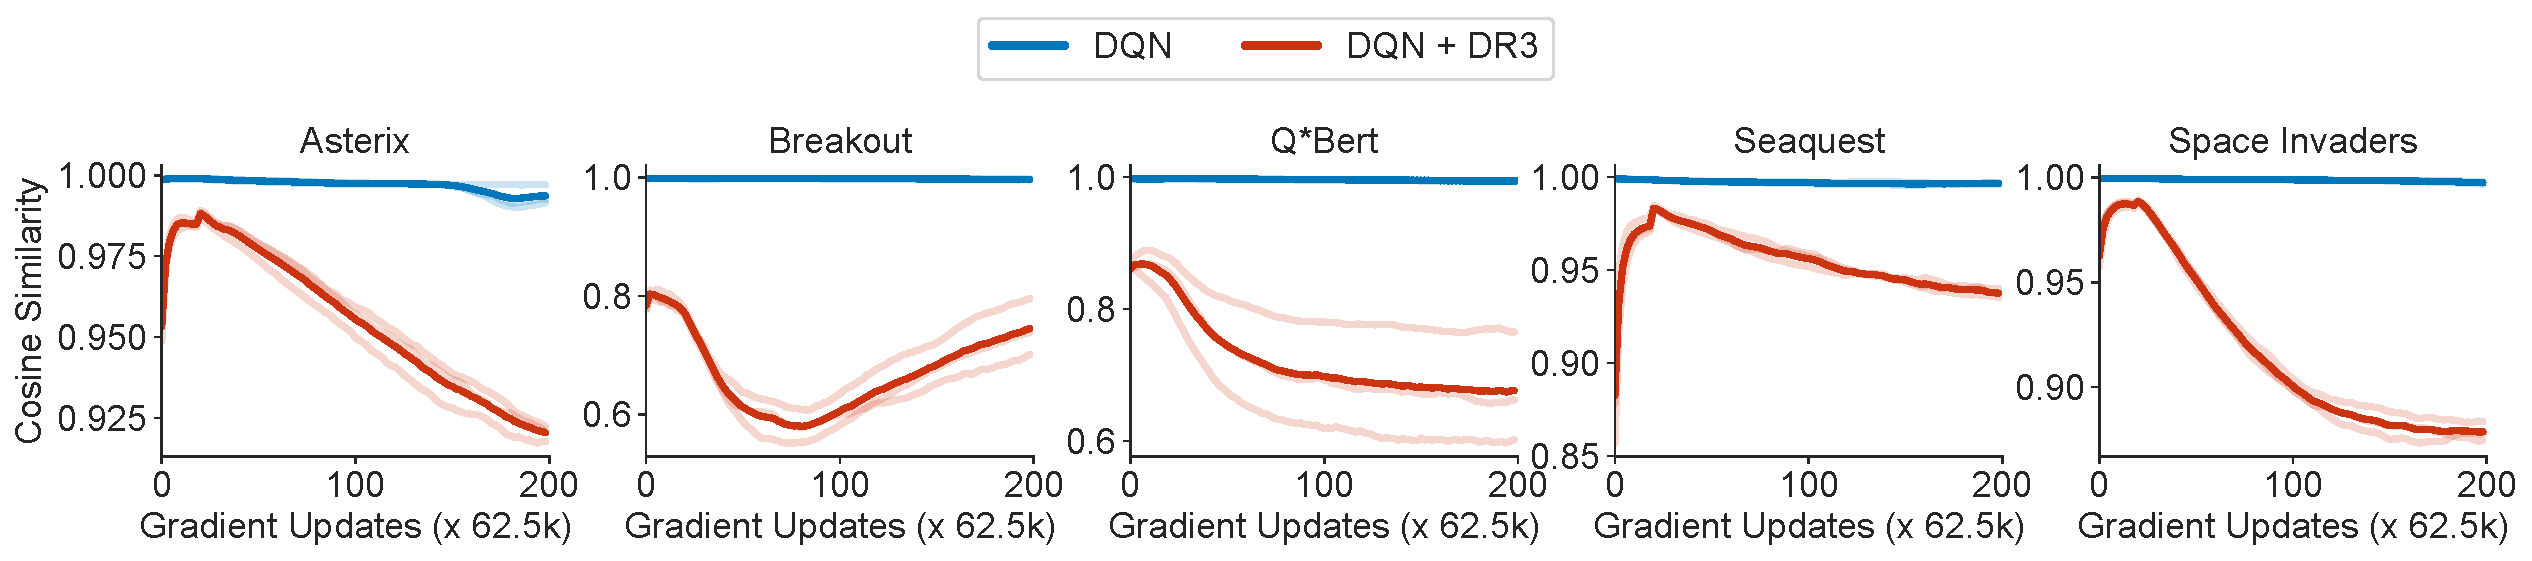
\includegraphics[width=0.99\textwidth]{rebuttal/rebuttal_dqn_cosine_sim_value_final_rebuttal.pdf}
    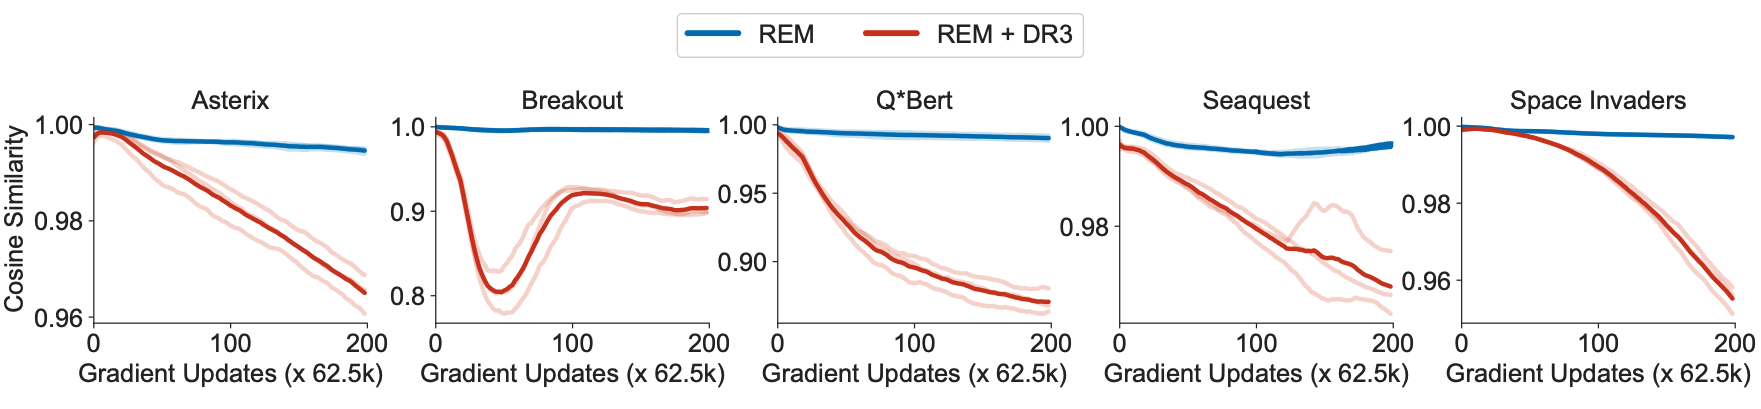
\includegraphics[width=0.99\textwidth]{rebuttal/rem_cosine.png}
    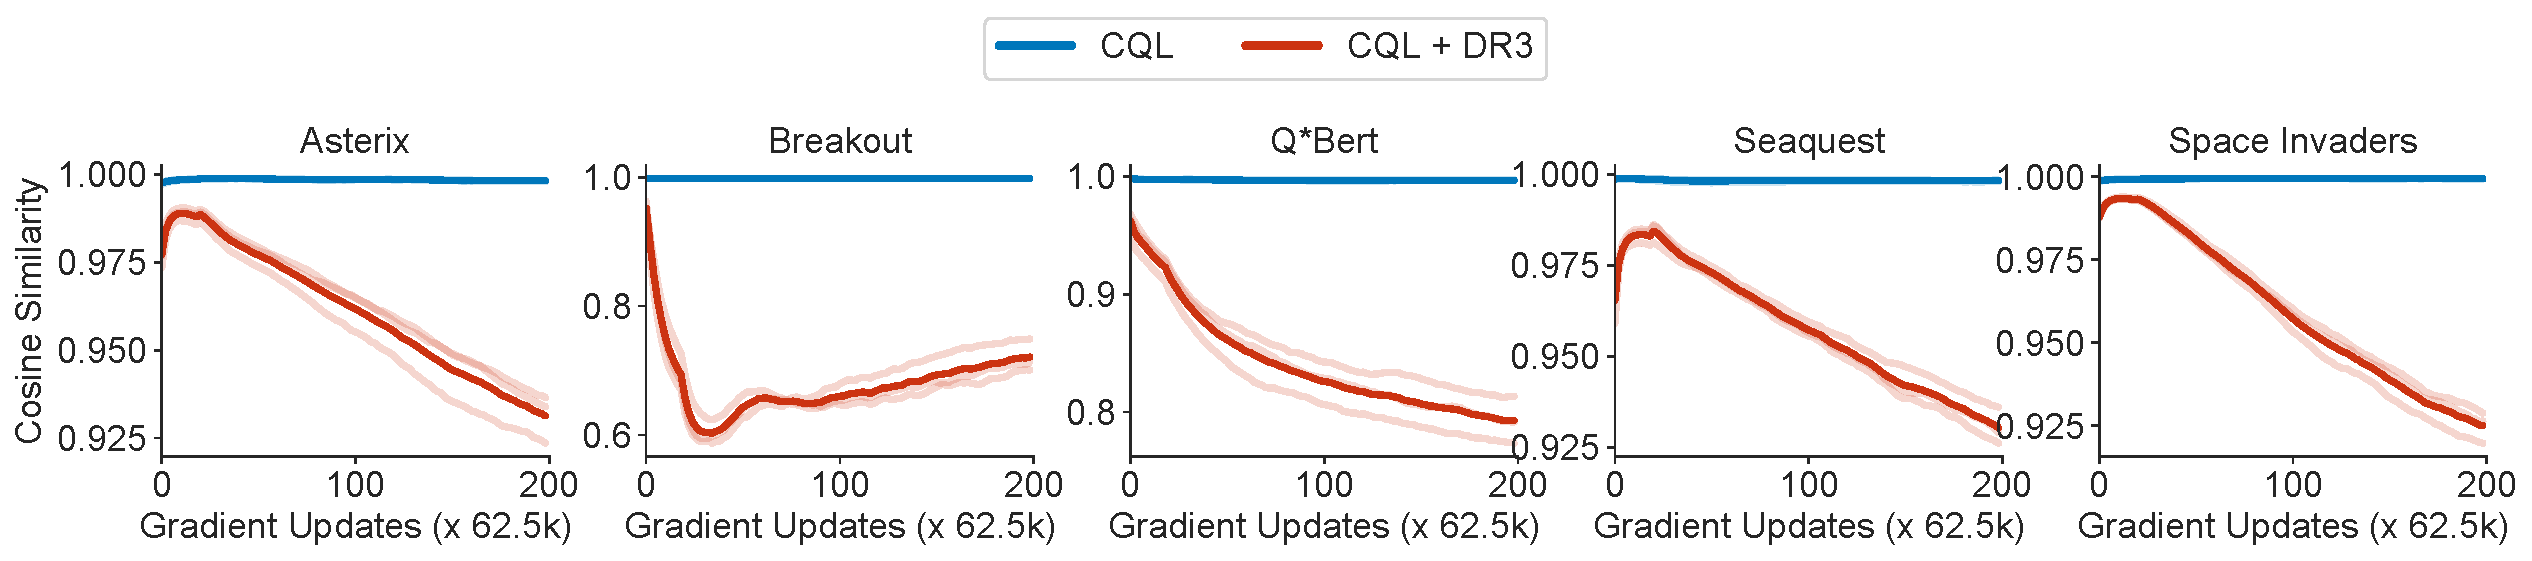
\includegraphics[width=0.99\linewidth]{rebuttal/rebuttal_cql_cosine_sim_value_final_rebuttal.pdf}
    \vspace{-5pt}
    \caption{\footnotesize{\label{fig:atari_cosine} \rebuttal{\textbf{Cosine similarities of DQN, DQN + DR3, REM, REM + DR3 and CQL, CQL + DR3.} Note that DQN, REM and CQL attain close to 1 cosine similarities, and addition of DR3 does reduce the cosine similarities of consecutive state-action features.}}}
    \vspace{-0.25cm}
\end{figure}

\begin{figure}[t]
    \centering
    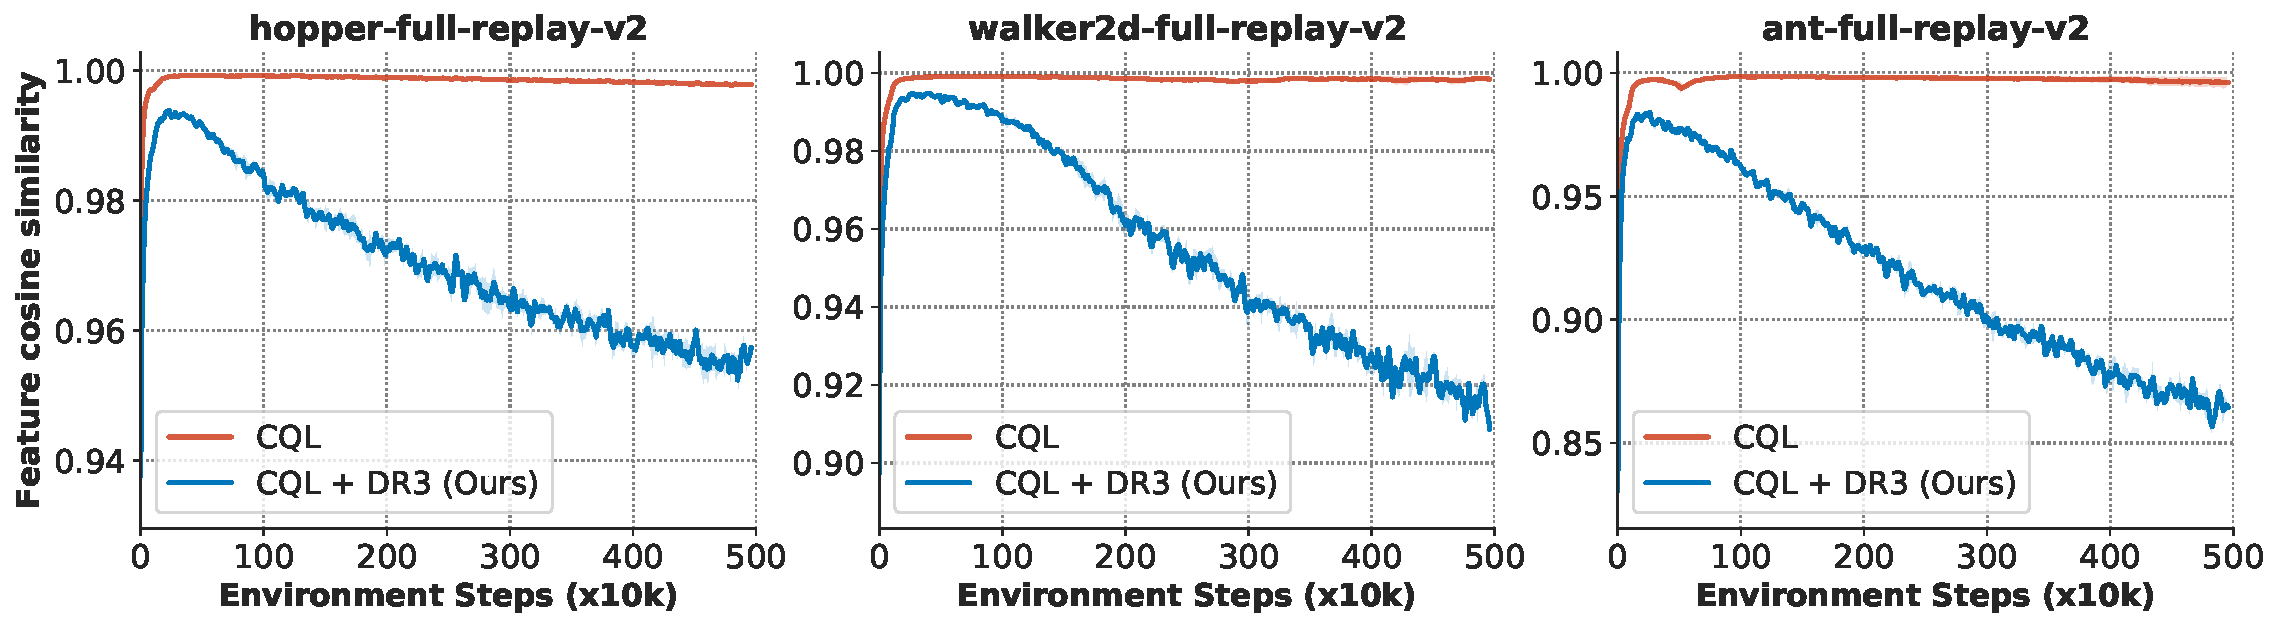
\includegraphics[width=0.9\textwidth]{rebuttal/offline_dr3_mujoco_envs_rebuttal_feat_cosine.pdf_Final.pdf}
    \vspace{-5pt}
    \caption{\footnotesize{\label{fig:mujoco_cosine} \rebuttal{\textbf{Cosine similarities of CQL and CQL + DR3 on MuJoCo domains.} Note that the cosine similarities of CQL grow to 1 and roughly stabilize for Ant and Walker2d, but start decreasing for Hopper. This happens despite the oscillatory trends in performance of CQL on Hopper~\ref{fig:mujoco_results_from_iup}. This means that a low cosine similarity need not imply poor performance, and DR3 can improve performance even when cosine similarity of base CQL is decreasing. We also notice that DR3 does actually reduce cosine similarity.}}}
    \vspace{-0.25cm}
\end{figure}


\subsection{\rebuttal{Stability of DR3 From a Good Solution}}
\label{app:cql_stability}
\rebuttal{In this appendix, we study the trend of CQL + DR3 when starting learning from a good initialization, which was studied in Figure~\ref{fig:stability}. As shown in Figure~\ref{fig:cql_stability}, while the performance for baseline CQL degrades significantly (from 5000 at initialization on Asterix, performance degrades to $\sim$2000 by 100 iterations for base CQL), whereas the performance of DR3 only moves from 5000 to $\sim$4300. A similar trend holds for Breakout. This means that the addition of DR3 does stabilize the learning relative to the baseline algorithm. Please note that we are not claiming that DR3 is unequivocally stable, but that improves stability relative to the base method.}

% \begin{figure}[t]
%     \centering
%     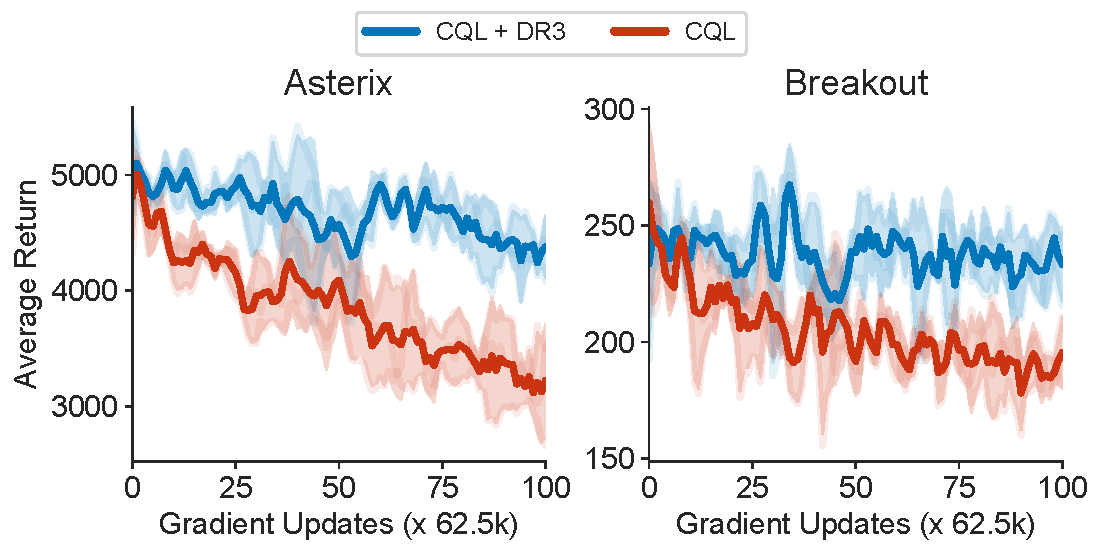
\includegraphics[width=0.45\textwidth]{rebuttal/figure_analysis_stability_with_without_dr3_cql.pdf} ~\vline~
%     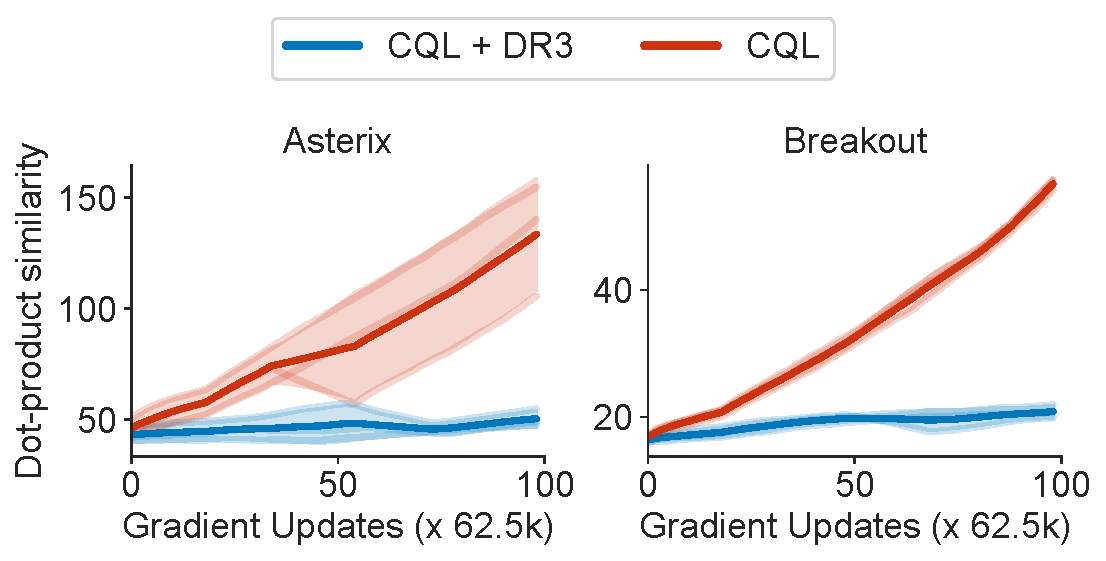
\includegraphics[width=0.45\textwidth]{rebuttal/figure_analysis_dot_product_stability_cql_vs_cql_dr3.pdf}
%     \vspace{-5pt}
%     \caption{\footnotesize{\label{fig:cql_stability} \rebuttal{\textbf{Running CQL + DR3 and CQL in the setup of Figure~\ref{fig:stability} to evaluate the stability of CQL + DR3 when starting training from a good solution.} Observe that the performance of base CQL decays quickly from the good solution, but CQL + DR3 is \emph{relatively} more stable. Additionally, the feature dot products for DR3 are much smaller compared to CQL.}}}
%     \vspace{-0.25cm}
% \end{figure}

\begin{figure}[t]
    \centering
    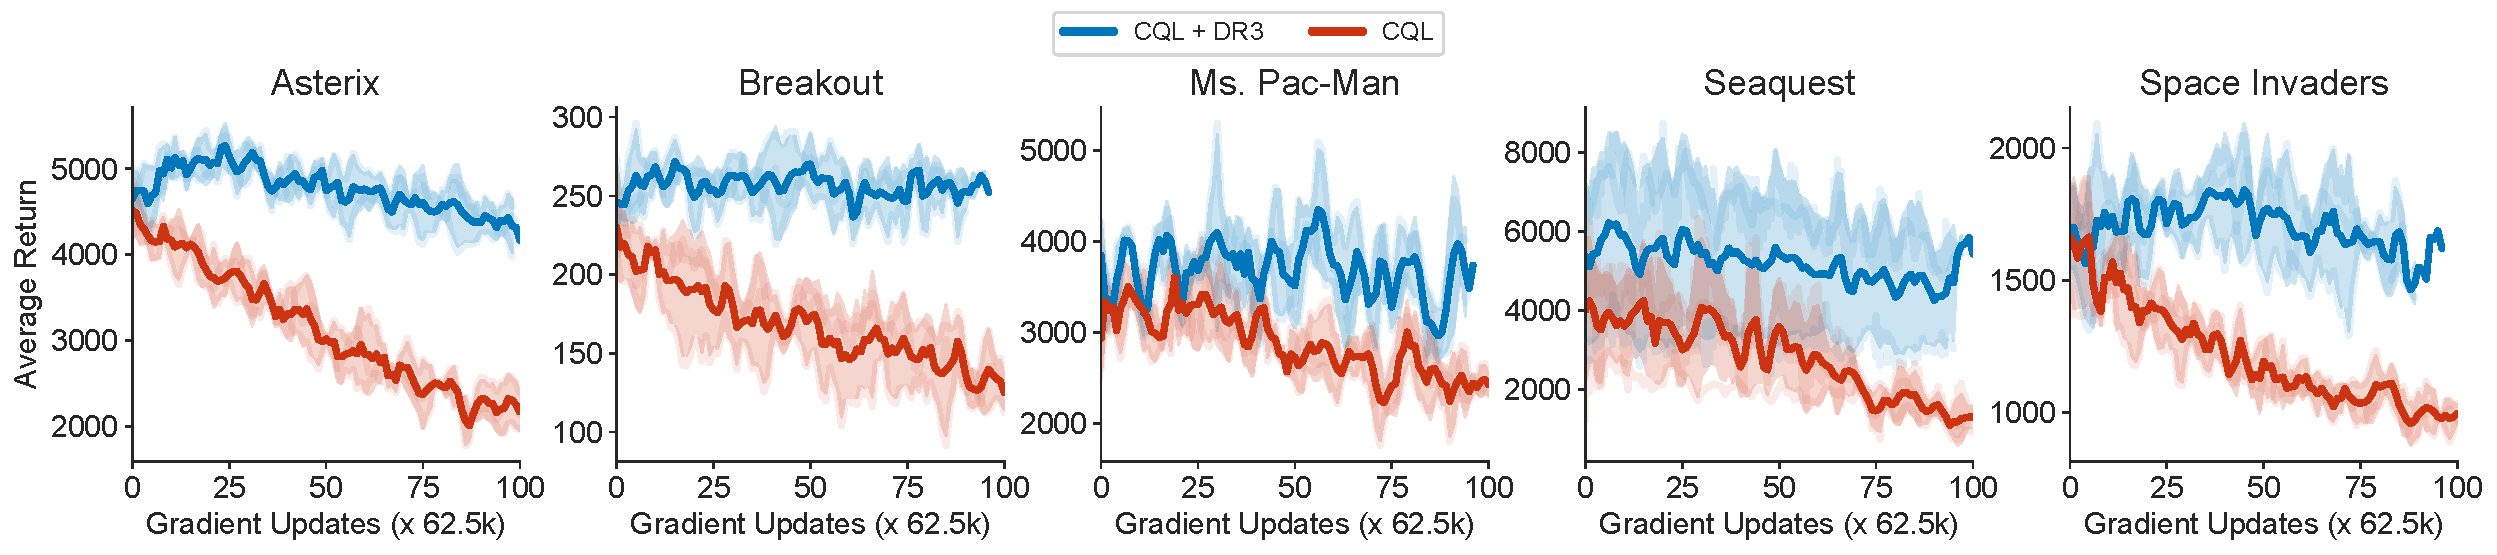
\includegraphics[width=0.99\textwidth]{rebuttal/figure_analysis_stability_five_games_final_cql_dr3.pdf}
    \vspace{-5pt}
    \caption{\footnotesize{\label{fig:cql_stability} \rebuttal{\textbf{Running CQL + DR3 and CQL in the setup of Figure~\ref{fig:stability} to evaluate the stability of CQL + DR3 when starting training from a good solution.} Observe that the performance of base CQL decays quickly from the good solution, but CQL + DR3 is \emph{relatively} more stable.}}}
    \vspace{-0.25cm}
\end{figure}

\begin{figure}[t]
    \centering
    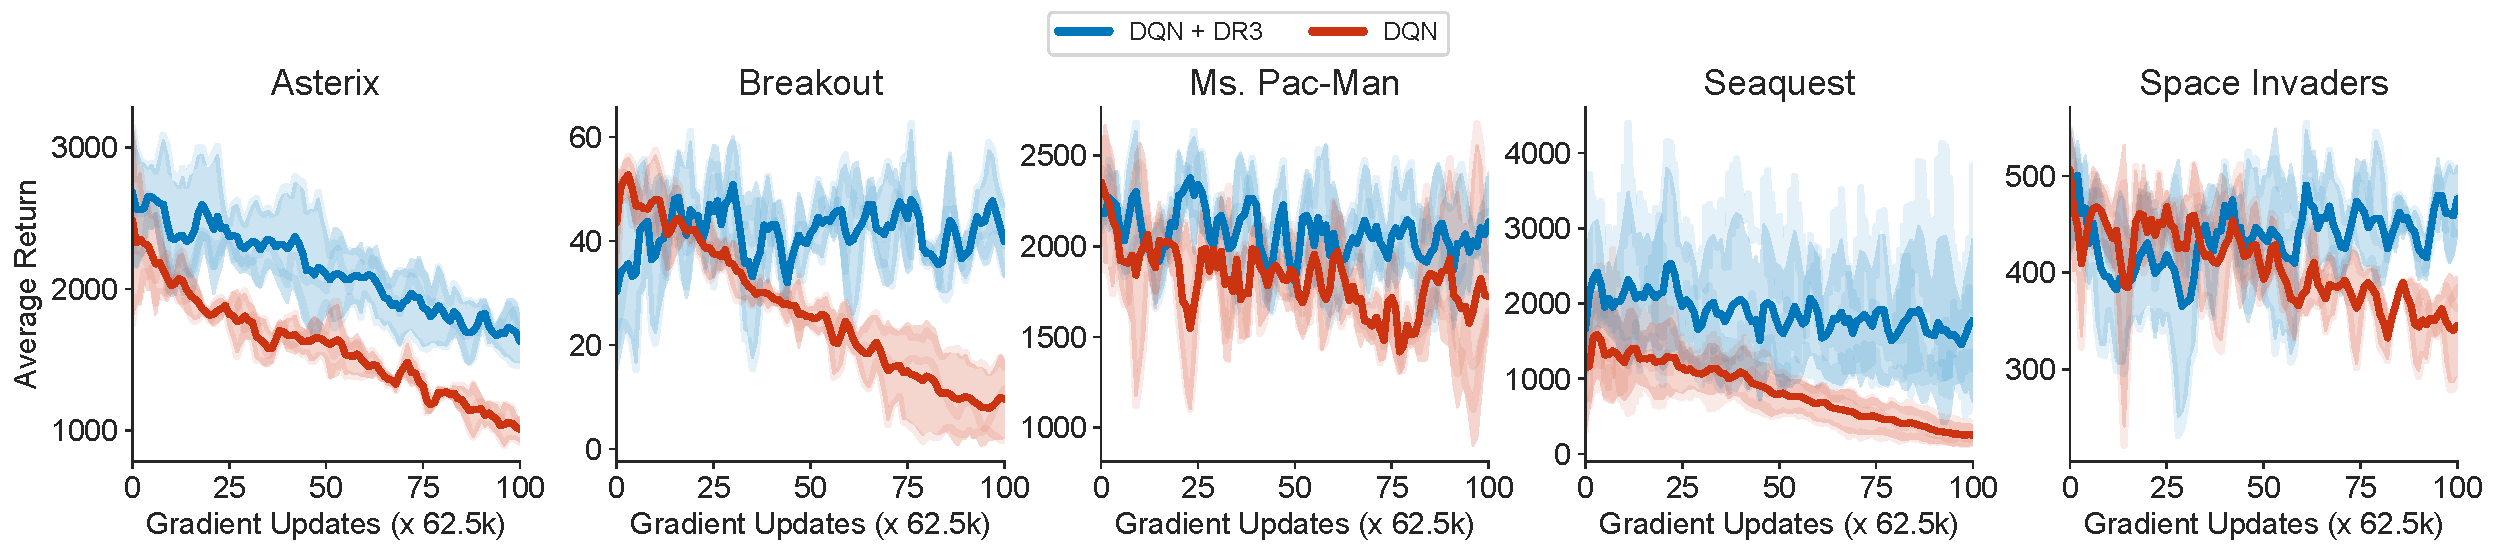
\includegraphics[width=0.99\textwidth]{rebuttal/figure_analysis_stability_five_games_final_dqn_dr3.pdf}
    \vspace{-5pt}
    \caption{\footnotesize{\label{fig:dqn_stability} \rebuttal{\textbf{Running DQN + DR3 and DQN in the setup of Figure~\ref{fig:stability} to evaluate the stability of DQN + DR3 when starting training from a good solution.} Observe that the performance of base DQN decays quickly from the good solution, but DQN + DR3 is \emph{relatively} more stable.}}}
    \vspace{-0.25cm}
\end{figure}

\vspace{-0.1cm}
\subsection{\rebuttal{Statistical Significance of DR3 and Franka Kitchen Results}}
\label{app:significance}

\begin{table}[h]
    % \begin{table}[t]
    % % \vspace{-0.8cm}
    \vspace{-0.05in}
    \fontsize{10}{8}\selectfont
    \centering
    \captionof{table}{\footnotesize{\textbf{Performance of CQL, CQL + \methodname\ after 2M gradient steps on the Franka Kitchen domains} averaged over 3 seeds. This is training for \textbf{6x} longer compared to CQL defaults. Observe that CQL + \methodname\ outperforms CQL at 2M steps, indicating is efficacy in preventing long term performance degradation.
    }}
    \label{tab:cql_kitchen}
    \vspace{-0.1in}
    \begin{tabular}{@{}lrr@{}}
    \toprule
    {\textbf{D4RL Task}} & CQL & CQL + \methodname \\
    \midrule
    % \texttt{kitchen-mixed} & 14.6 $\pm$ 20.5 & \textbf{37.0 $\pm$ 8.0} \\
    % \texttt{kitchen-partial} & 29.6 $\pm$ 19.6 & \textbf{43.5 $\pm$ 1.9}  \\
    % \texttt{kitchen-complete} & 22.3 $\pm$ 17.5 & 24.8 $\pm$ 15.3 \\
    \texttt{kitchen-mixed} & 27.67 $\pm$ 12.66 & \textbf{37.00 $\pm$ 11.53} \\
    \texttt{kitchen-partial} & 20.67 $\pm$ 15.57 & \textbf{40.67 $\pm$ 4.04}  \\
    \texttt{kitchen-complete} & 28.00 $\pm$ 14.73 & \textbf{38.67 $\pm$ 6.66} \\
    \bottomrule
    \end{tabular}
    % \vspace{cm}
\end{table}
We present the results comparing CQL and CQL+DR3 on the Franka Kitchen tasks from D4RL in Table~\ref{tab:cql_kitchen}. Observe that CQL+DR3 outperforms CQL, and to test the statistical significance of these results, we analyze the probability of improvement of CQL+DR3 over CQL next.

% \vspace{-0.5cm}
\begin{figure}[H]
    \centering
    \vspace{-0.15cm}
    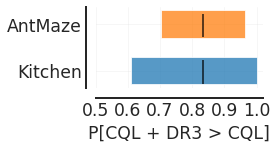
\includegraphics[width=0.4\linewidth]{rebuttal/statistical_significance.png}
    \vspace{-0.2cm}
    \caption{\label{fig:significance} \footnotesize{\rebuttal{\textbf{Statistical significance of the results of CQL + DR3 vs CQL (Table~\ref{tab:cql_d4rl}) as measured by average probability of improvement~\citep{agarwal2021precipice},} with stratified bootstrap confidence intervals for this statistic. Since the lower CI for this statistic is $> 0.5$, CQL + DR3 \textbf{significantly} improves over base CQL, and since the mean and upper CI are $\geq 0.75$, this improvement is also \textbf{meaningful}.}}} 
    \vspace{-0.4cm}
\end{figure}

\rebuttal{In order to assess the statistical significance of our D4RL Antmaze and Kitchen results, we follow the recommendedations by \citet{agarwal2021precipice} for comparing deep RL algorithms considering their statistical uncertainties. Specifically, we computed the average probability of improvement~\citep{agarwal2021precipice} of CQL + DR3 over CQL on the antmaze and kitchen domains, and we find that DR3 \textbf{does} significantly and meaningfully improve over CQL on both the Kitchen and AntMaze domains. Before presenting the results, let us first describe the metric we compute.}

% \vspace{-0.1cm}
\rebuttal{\textbf{Probability of improvement and statistical significance}. For two given algorithms $\mathsf{Alg}_1$ and $\mathsf{Alg}_2$, and runs $X_{k,1}, X_{k,2}, \cdots, X_{k,m}$ from $\mathsf{Alg}_1$ and runs $Y_{k,1}, Y_{k,2}, \cdots, Y_{k,n}$ from $\mathsf{Alg}_2$ on task $k$, the probability of improvement of $\mathsf{Alg}_1$ over $\mathsf{Alg}_2$ is given by $P(\mathsf{Alg}_1 > \mathsf{Alg}_2) = \frac{1}{K} \sum_{k=1}^{K} P(\mathsf{Alg}^k_1 > \mathsf{Alg}^k_2)$. The probability of improvement on a given task $k$,   $P(\mathsf{Alg}^k_1 > \mathsf{Alg}^k_2)$ is computed using the Mann-Whitney U-statistic and is given by:}
\vspace{-0.2cm}
\rebuttal{
\begin{align*}
   P(\mathsf{Alg}^k_1 > \mathsf{Alg}^k_2) = \frac{1}{M N} \sum_{i=1}^{M}\sum_{j=1}^{N}S(X_{k,i}, Y_{k, j})\quad \text{where}\quad
S(x,y)={\begin{cases}1,&{\text{if }}y<x,\\{\tfrac {1}{2}},&{\text{if }}y=x,\\0,&{\text{if }}y>x.\end{cases}}\label{eq:prob_improve}
\end{align*}
\vspace{-0.05cm}
}


\rebuttal{\!$\mathsf{Alg}_1$ leads to statistically \emph{significant} improve over $\mathsf{Alg}_2$ if the lower CI for $\mathsf{P} (\mathsf{Alg}_1 > \mathsf{Alg}_2)$ is larger than 0.5. Per the Neyman-Pearson statistical testing criterion in \citet{bouthillier2021accounting}, $\mathsf{Alg}_1$ leads to statistically \emph{meaningful} improvement over $\mathsf{Alg}_2$  if the upper confidence interval~(CI) of $\mathsf{P} (\mathsf{Alg}_1 > \mathsf{Alg}_2)$ is larger than 0.75.} 

\rebuttal{Figure~\ref{fig:significance} presents the value of $\mathsf{P} (\text{CQL + DR3} > \text{CQL})$ on the AntMaze and Kitchen domains at 2M gradient steps along with the 95\% CI for this statistic. DR3 improves over CQL on the AntMaze domains with probability \textbf{0.83} with 95\% CI (0.7, 0.96) and on the Kitchen domains with probability \textbf{0.8} with 95\% CI (0.6, 1.0). These values pass the criterion of being both statistically significant and meaningful per the above definitions, implying that DR3 does significantly and meaningfully improve upon CQL on these domains.}